\documentclass[letterpaper,twocolumn,10pt]{article}
\usepackage{jsys}

% Disable a warning related to \nonfrenchspacing
\microtypecontext{spacing=nonfrench}

% to be able to draw some self-contained figs
\usepackage{algorithmicx}
\usepackage{algorithm}
\usepackage{algpseudocode}
\usepackage{amsthm}
\usepackage{booktabs}
\usepackage{bpaxos}
\usepackage{drawings}
\usepackage{lipsum}
\usepackage{pervasives}
\usepackage{subcaption}
\usepackage{tikz}
\usepackage{wrapfig}
\usetikzlibrary{backgrounds}
\usetikzlibrary{calc}
\usetikzlibrary{decorations.pathreplacing}
\usetikzlibrary{patterns}
\usetikzlibrary{positioning}

% Remove the "end if" from algorithmicx. See [1].
%
% [1]: https://tex.stackexchange.com/a/53518
\algtext*{EndIf}
\algtext*{EndFor}

% Custom upon ... do block.
\algblockdefx[Upon]{Upon}{EndUpon}
  [1]{\textbf{upon} #1 \textbf{do}}
  {end}
\algtext*{EndUpon}

% Custom State: block.
\algnewcommand{\algorithmicstate}{\textbf{State:}}
\algnewcommand{\GlobalState}{\item[\algorithmicstate]}

\newcommand{\BipartisanPaxos}{Pinata Paxos}
\newcommand{\BPaxos}{PPaxos}
\newcommand{\msgfont}[1]{\textsc{#1}}
\newcommand{\msg}[2]{\msgfont{#1}$\langle #2 \rangle$}
\newcommand{\PhaseIA}[1]{\msgfont{Phase1A}\langle{#1}\rangle}
\newcommand{\PhaseIB}[3]{\msgfont{Phase1B}\langle{#1, #2, #3}\rangle}
\newcommand{\PhaseIIA}[2]{\msgfont{Phase2A}\langle{#1, #2}\rangle}
\newcommand{\PhaseIIB}[1]{\msgfont{Phase2B}\langle{#1}\rangle}

\newcommand{\maj}[1]{\textsf{maj}(#1)}

% Uncomment the following line if you want the columns of the last page equal in
% size. But note that doing so may cause issues with some document-generating
% tools.
% \usepackage{flushend}


\begin{document}

%don't want date printed
\date{}

% make title bold and 14 pt font (Latex default is non-bold, 16 pt)
\title{TODO}

%for single author (just remove % characters)
\author{{\rm Your N.\ Here}\\
  Your Institution
  \and
  {\rm Second Name}\\
  Second Institution
  % copy the following lines to add more authors \and {\rm Name}\\
  % Name Institution
} % end author


\maketitle

% Disable header and footer on the from page
\thispagestyle{empty}

% {\begin{abstract}
  In this paper, we present a family of state machine replication protocols
  inspired by Fast Paxos~\cite{lamport2006fast}, EPaxos~\cite{moraru2013there},
  and Caesar~\cite{arun2017speeding}. The protocols are called Bipartisan
  Paxos, Unanimous Bipartisan Paxos, and Majority Commit Bipartisan Paxos.
\end{abstract}

}
% {\section{Introduction}
State machine replication protocols like MultiPaxos~\cite{lamport1998part,
lamport2001paxos} and Raft~\cite{ongaro2014search} allow a state machine to be
executed in unison across a number of machines, despite the possibility of
faults. Today, state machine replication is pervasive. Nearly every strongly
consistent distributed system is implemented with some form of state machine
replication~\cite{corbett2013spanner, thomson2012calvin, hunt2010zookeeper,
burrows2006chubby, baker2011megastore, cockroach2019website, cosmos2019website,
tidb2019website, yugabyte2019website}.

MultiPaxos is one of the oldest and one of the most widely used state machine
replication protocols. Despite its popularity, MultiPaxos doesn't have optimal
throughput or optimal latency. In MultiPaxos, \emph{every} command is sent to a
single elected leader. This leader becomes a bottleneck, limiting the
throughput of the protocol. Moreover, when a client sends a command to the
leader, it must wait at least two round trips before receiving a response. This
is twice as long as the theoretical minimum of one round
trip~\cite{lamport2006lower}.

An enormous number of state machine replication protocols have been proposed to
address MultiPaxos' suboptimal performance. These protocols use sophisticated
techniques that increase MultiPaxos' throughput, decrease its latency,
or both. For example, techniques like
  deploying multiple leaders~\cite{mao2008mencius, moraru2013there,
  arun2017speeding},
  %
  using flexible quorum sizes~\cite{howard2016flexible, nawab2018dpaxos}, and
  %
  separating the control path from the data path~\cite{biely2012s}
increase MultiPaxos' throughput. Techniques like
  bypassing the leader~\cite{lamport2006fast, ports2015designing, li2016just}
  and
  %
  speculatively executing commands~\cite{ports2015designing, li2016just,
  park2019exploiting}
decrease MultiPaxos' latency. Techniques like
  exploiting commutativity~\cite{lamport2005generalized, moraru2013there,
  arun2017speeding, park2019exploiting}
do both.

Many of these sophisticated protocols try to \emph{simultaneously} increase
throughput and decrease latency, using a combination of the techniques
described in the previous paragraph. For example, NoPaxos ``outperforms both
latency- and throughput-optimized protocols on their respective
metrics''~\cite{li2016just}, whereas EPaxos achieves ``optimal commit latency
in the wide-area'' while ``achieving high throughput''~\cite{moraru2013there}.

Trying to increase throughput \emph{and} decrease latency is a complex
endeavor. Protocols that aim to improve \emph{both} are forced to implement
multiple of the techniques mentioned above in a single protocol. In isolation,
these techniques are challenging to implement. When superimposed, they become
even harder. The techniques have to be sewn together in subtle and intricate
ways. These protocols become increasingly complex, with different components
tightly integrated together. Eventually, it becomes difficult to understand any
single piece of a protocol without first having a strong grasp on
the protocol as a whole. Paradoxically, newcomers must first understand the
protocol before they can begin to understand it!

In this paper, we take a different approach. Instead of chasing both throughput
\emph{and} latency, \textbf{we trade off a bit of latency for modularity}. We
present Bipartisan Paxos (BPaxos), a state machine replication protocol that
sacrifices optimal latency for a modular design. BPaxos is composed of a number
of independent modules. Each module can be understood in isolation and composed
together in a straightforward way to form the protocol as a whole. BPaxos'
modular design leads to simplicity and (surprisingly) higher throughput.

% Unfortunately, these advanced techniques don't come for free. They
% significantly complicate the protocols. MultiPaxos is already notoriously
% difficult to understand~\cite{van2015paxos, ongaro2014search}, and these
% sophisticated protocols make MultiPaxos seem like a piece of cake. In fact,
% these protocols can be so complex that bugs in the protocols can go
% undiscovered for years. Generalized Paxos~\cite{lamport2005generalized} and
% Zyzyva~\cite{kotla2007zyzzyva} had bugs that went undiscovered for seven and
% ten years respectively~\cite{sutra2011fast, abraham2017revisiting}. In writing
% this paper, we discovered bugs ourselves in EPaxos~\cite{moraru2013there} and
% DPaxos~\cite{nawab2018dpaxos} six years and one year after their publications
% respectively.
% %
% \TODO[mwhittaker]{Add bugs to appendix and reference appendix.}
%
% Worse yet, the vast majority of these protocols are incomplete. Many omit
% features, like garbage collection, that are necessary to implement the
% protocols in practice. These omitted features would add even more complexity to
% the already complex protocols.
%
% In this paper, we present a new state machine replication protocol called
% Bipartisan Paxos, or BPaxos for short. BPaxos is simpler, has higher
% throughput, and is more complete than state of the art replication protocols.

\paragraph{Simplicity}
It's hard to quantify the ``complexity'' of a protocol, how hard it is for
someone to understand. But, where there's smoke there's fire, and if we look at
protocols closely enough, we start to see smoke. Generalized
Paxos~\cite{lamport2005generalized} was published in 2005. Seven years later,
someone found a bug in one of its assumptions~\cite{sutra2011fast}.
Zyzyva~\cite{kotla2007zyzzyva}, a Byzantine replication protocol, was published
in 2007. Ten years later, the authors published a paper noting that the
protocol is actually unsafe~\cite{abraham2017revisiting}. In writing this
paper, we discovered bugs ourselves in two other protocols,
EPaxos~\cite{moraru2013there} and DPaxos~\cite{nawab2018dpaxos}, which we
confirmed with the protocols' authors. These long undiscovered bugs suggest
that protocols chasing high throughput and low latency are often forced to
sacrifice simplicity.
\TODO[mwhittaker]{Add bugs to appendix and reference.}

BPaxos' modular design makes it easier to understand. Each module can be
understood and proven correct in isolation, allowing newcomers to understand
the protocol piece by piece.
% Say something about how some modules, like consensus, implement well known
% abstractions and how we can take existing protocols and plug them in. E.g.,
% we use Paxos to implement consensus. Other protocols like EPaxos and Caesar
% implement their own consensus and have to prove everything is correct.

% Most of the sophisticated state machine replication protocols try to
% simultaneously achieve high throughput \emph{and} low latency. The key insight
% that enables BPaxos' simplicity is that trading off a bit of latency can
% significantly reduce complexity. BPaxos exploits this insight to achieve
% simplicity in three ways.
% \TODO[mwhittaker]{Quantify what we mean by ``a bit of latency''.}
%
% First, \textbf{BPaxos is modular.} Many protocols couple and co-locate
% components together to decrease latency. BPaxos takes the opposite approach and
% instead decouples the protocol into a number of independent modules. Each
% module can be understood in isolation, making the protocol understandable piece
% by piece.
%
% Second, \textbf{BPaxos leverages existing protocols.} Because BPaxos is
% composed of a number of independent modules, BPaxos is able to use existing,
% well known protocols to implement some modules. This way, BPaxos avoids
% reimplementing the wheel. For example, BPaxos uses Paxos to implement a
% consensus module.
%
% Third, \textbf{BPaxos avoids fast paths.} Most sophisticated state machine
% replication protocols, starting with Fast Paxos~\cite{lamport2006fast}, have a
% fast path and a slow path. The protocols optimistically attempt to take the
% fast path, but are sometimes forced to revert to the slow path.  Fast paths
% decrease latency in the best case but complicate parts of the protocols (e.g.,
% the recovery procedure). BPaxos does not use fast paths, again sacrificing
% latency for simplicity.

\paragraph{High Throughput}
We initially modularized BPaxos to trade off latency for simplicity.
Surprisingly, we found that modularizing the protocol also led to high
throughput. Many existing protocols pack a handful of logical processes onto a
single physical process. For example, a single process may play the role of a
Paxos proposer, acceptor, and state machine replica. This co-location leads to
lower latency. Messages sent between logical nodes do not have to traverse the
network if the two nodes are physically co-located.

BPaxos does \emph{not} couple logical processes together. Instead, we found
that by decoupling the protocol, we are able to significantly increase the
protocol's throughput using a simple trick: scaling. We perform a bottleneck
analysis on the protocol's components. Once we identify the bottleneck
component, we simply scale up the component until it is no longer the
bottleneck.

For example, if our protocol consisted of proposers, acceptors, and state
machine replicas and if we concluded that the proposers were the bottleneck, we
would simply add more proposers. This straightforward scaling is not so easy to
do in tightly coupled protocols. If every node is a proposer, an acceptor, and
a state machine replica, for example, then adding more proposers also
introduces more acceptors and more replicas. Adding more of a certain component
can actually slow down a protocol instead of speeding it up. For example, more
acceptors lead to larger quorums which lead to slower protocols.

\paragraph{Completeness}
Every node in a state machine replication protocol stores some state. For
example, MultiPaxos acceptors store a collection of votes and round numbers,
and MultiPaxos replicas store a log of state machine commands. This state grows
over time and must be garbage collected in order to avoid exhausting a
protocol's physical memory.

Garbage collection algorithms exist for protocols like MultiPaxos and Raft, but
many sophisticated state machine replication protocols are introduced without
detailing a garbage collection algorithm~\cite{%
  moraru2013there, % EPaxos
  arun2017speeding, % Caesar
  zhang2018building, % TAPIR
  mu2016consolidating % Janus
}. This leaves practitioners and protocol implementors responsible for piecing
together how to implement garbage collection correctly. Unfortunately, these
garbage collection algorithms are subtle and hard to get right. In this paper,
we detail a complete garbage collection algorithm for BPaxos. These details are
essential to implement BPaxos completely, and we believe they are also useful
to understand how to implement garbage collection in other sophisticated state
machine replication protocols.

In summary, we present the following contributions:
\begin{itemize}
  \item
    We introduce Bipartisan Paxos: a modular state machine replication protocol
    that trades off a bit of latency for a significant increase in simplicity.
  \item
    We describe how BPaxos' modularity leads to a straightforward form of
    scaling that yields high throughput without added complexity.
  \item
    We detail a garbage collection algorithm for BPaxos, a protocol that also
    sheds light on how to perform garbage collection in similar protocols.
\end{itemize}

% \begin{itemize}
%   \item consensus is important and pervasive
%   \item multipaxos is the most commonly used everywhere
%   \item multipaxos doesn't have the best throughput or latency. single master
%     means throughput bottleneck. two round trip from client not optimal either.
%   \item as a result, a ton of protocols attempting to improve on multipaxos
%     using a ton of techniques, (fast quorums, generalized, speculative exec,
%     multimaster, flexible quorum sizes, etc)
%   \item
%     multipaxos is complicated and these fancier protocols are even more complicated
%   \item Generalized, Paxos, Zyzyva, EPaxos, DPaxos all buggy
%   \item complex protocols are discouraging to implement in practice and easy to get wrong
%   \item moreover, these protocols are incomplete, leaving out essential features like gc
%   \item
%   \item in this paper, we present a new consensus protocol that is simpler than
%     state of the art, has higher throughput than state of the art, and is more
%     complete than state of the art.
%   \item
%   \item novelty 1: simplicity
%   \item --- insight 1: trade latency for simplicity
%   \item --- Paxos has a bad rep for being complicated
%   \item --- Fancier variants are even more complicated
%   \item --- modularity, re-use, no fast paths
%   \item --- emphasize not simpler than multpaxos but simpler than alternatives
%   \item novelty 2: high throughput
%   \item --- insight 2: decouple protocols leads to a huge number of benefits
%   \item --- decoupling and modularity reduce latency but improve throughput
%   \item --- decoupling helps identify throughput bottlenecks and scale the protocol
%   \item --- We can get state of the art throughput without adding complexity
%   \item novelty 3: garbage collection
%   \item --- gc is necessary. without it, processes run out of memory
%   \item --- mp has gc
%   \item --- all other protocols do not discuss it
%   \item --- gc is considerably more complex in these scenarios
%   \item --- we are the first to present gc
%   \item --- gc simplified by modular architecture
% \end{itemize}
%
%
%
%
%
%
%
%
% \begin{itemize}
%   \item Introduction
%
%   \item Background
%     \begin{itemize}
%       \item MultiPaxos
%     \end{itemize}
%
%   \item Bipartisan Paxos
%     \begin{itemize}
%       \item Main idea overview
%       \item Protocol overview with figure
%       \item Dependency service
%       \item Consensus Service
%       \item Replicas
%       \item BPaxos Nodes
%       \item Example
%       \item Full pseudo-code
%       \item Recovery
%     \end{itemize}
%
%   \item Scaling
%     \begin{itemize}
%       \item Other protocols tightly coupled
%       \item Our protocol decoupled, already gives boost
%       \item Bottleneck analysis
%       \item Scale to eliminate bottleneck
%     \end{itemize}
%
%   \item Garbage Collection
%     \begin{itemize}
%       \item Leaders
%       \item Acceptors and Proposers
%       \item Dependency service, new dep service properties
%       \item Replica
%     \end{itemize}
%
%   \item Practical Considerations
%     \begin{itemize}
%       \item Client table
%       \item Dependency compaction
%       \item
%     \end{itemize}
%
%   \item Evaluation
%     \begin{itemize}
%       \item
%         latency throughput of protocol in lan vs epaxos and paxos (for various
%         params)
%       \item
%         same graph as above without decoupling and without scaling to show
%         effects
%       \item
%         latency throughput of protocols in lan with batching
%       \item
%         graphs to show garbage collection effects on throughput (makes it
%         jittery), memory usage over time with projection on how long before
%         running out.
%       \item
%         latency throughput of protocol in WAN to show that it's actually not
%         great
%     \end{itemize}
%
%   \item Related work
%     \begin{itemize}
%       \item EPaxos
%       \item Caesar
%       \item Mencius
%       \item PODC announcement
%       \item SPaxos (decoupling)
%       \item Multithreaded paxos (essentially decoupling)
%       \item all other papers on gc
%     \end{itemize}
%
%   \item Appendix
%     \begin{itemize}
%       \item Execute conflicting commands in same order equivalent to gen paxos
%       \item Bugs in other protocols.
%       \item TLA+ specification of protocol.
%     \end{itemize}
% \end{itemize}
}
{\section{Background}

\subsection{Paxos}
Assume we have a number of clients, each with a value that they would like to
propose. The \defword{consensus} problem is for all members to agree on a
single value among the proposed values. A consensus protocol is a protocol that
implements consensus. Clients propose commands by sending them to the protocol.
The protocol eventually chooses a single one of the proposed values and returns
it to the clients.

Paxos~\cite{lamport1998part, lamport2001paxos} is one of the oldest and most
well studied consensus protocols. We will see later that BPaxos uses Paxos to
implement consensus, so it is important to be familiar with \emph{what} Paxos
is. Fortunately though, BPaxos treats Paxos like a black box, so we do not have
to concern ourselves with \emph{how} Paxos works.

\subsection{MultiPaxos}
Whereas consensus protocols like Paxos agree on a \emph{single} value,
\defword{state machine replication} protocols like MultiPaxos agree on a
\emph{sequence} of values called a log.  A state machine replication protocol
involves some number of replicas of a state machine, with each state machine
beginning in the same initial state. Clients propose commands to the
replication protocol, and the protocol orders the commands into an agreed upon
log that grows over time. Replicas execute entries in the log in prefix order.
By beginning in the same initial state and executing the same commands in the
same order, all the replicas are guaranteed to remain in sync.

MultiPaxos~\cite{van2015paxos} is one of the earliest and most popular state
machine replication protocols. MultiPaxos uses one instance of Paxos for every
log entry, agreeing on the log entries one by one. For example, it runs one
instance of Paxos to agree on the command chosen in log entry 0, one instance
for log entry 1, and so on. Over time, more and more commands are chosen, and
the log of chosen commands grows and grows. MultiPaxos replicas execute
commands as they are chosen, taking care not to execute the commands out of
order.

For example, consider the example execution of a MultiPaxos replica depicted in
\figref{ExampleMultiPaxosExecution}. The replica implements a key-value store
with keys $a$ and $b$. First, the command $a \gets 0$ (i.e.\ set $a$ to $0$) is
chosen in log entry $0$ (\figref{ExampleMultiPaxosExecutionA}), and the replica
executes the command (\figref{ExampleMultiPaxosExecutionB}). Then, the command
$a \gets b$ is chosen in log entry $2$ (\figref{ExampleMultiPaxosExecutionC}).
The replica cannot yet execute the command, because it must first execute the
command in log entry $1$, which has not yet been chosen
(\figref{ExampleMultiPaxosExecutionD}).  Finally, $b \gets 0$ is chosen in log
entry $1$ (\figref{ExampleMultiPaxosExecutionE}), and the replica can execute
the commands in both log entries $1$ and $2$. Note that the replica executes
the log in prefix order, waiting to execute a command if previous commands have
not yet been chosen and executed.

{\newlength{\logentryinnersep}
\setlength{\logentryinnersep}{2pt}
\newlength{\logentrylinewidth}
\setlength{\logentrylinewidth}{1pt}
\newlength{\logentrywidth}
\setlength{\logentrywidth}{\widthof{\scriptsize$a \gets 1$}+2\logentryinnersep}
\newcommand{\logindexcolor}{flatred}
\newcommand{\cmdi}{$a \gets 0$}
\newcommand{\cmdii}{$b \gets 0$}
\newcommand{\cmdiii}{$a \gets b$}

\tikzstyle{logentry}=[draw,
                      font=\scriptsize,
                      inner sep=\logentryinnersep,
                      line width=\logentrylinewidth,
                      minimum height=\logentrywidth,
                      minimum width=\logentrywidth]
\tikzstyle{executed}=[fill=gray, opacity=0.2, draw opacity=1, text opacity=1]
\tikzstyle{logindex}=[\logindexcolor]

\newcommand{\rightof}[1]{-\logentrylinewidth of #1}

\newcommand{\multipaxoslog}[6]{%
  \node[logentry, label={[logindex]90:0}, #2] (0) {#1};
  \node[logentry, label={[logindex]90:1}, right=\rightof{0}, #4] (1) {#3};
  \node[logentry, label={[logindex]90:2}, right=\rightof{1}, #6] (2) {#5};
}

\begin{figure}[ht]
  \begin{subfigure}[t]{0.45\columnwidth}
    \centering
    \begin{tikzpicture}
      \multipaxoslog{\cmdi}{}%
                    {}{}%
                    {}{}
    \end{tikzpicture}
    \caption{%
      \cmdi{} is chosen in entry $\textcolor{\logindexcolor}{0}$.
    }
    \figlabel{ExampleMultiPaxosExecutionA}
  \end{subfigure}\hspace{0.1\columnwidth}%
  \begin{subfigure}[t]{0.45\columnwidth}
    \centering
    \begin{tikzpicture}
      \multipaxoslog{\cmdi}{executed}%
                    {}{}%
                    {}{}
    \end{tikzpicture}
    \caption{%
      \cmdi{} is executed.
    }
    \figlabel{ExampleMultiPaxosExecutionB}
  \end{subfigure}

  \vspace{2pt}\textcolor{flatgray}{\rule{\columnwidth}{0.4pt}}

  \begin{subfigure}[t]{0.45\columnwidth}
    \centering
    \begin{tikzpicture}
      \multipaxoslog{\cmdi}{executed}%
                    {}{}%
                    {\cmdiii}{}
    \end{tikzpicture}
    \caption{%
      \cmdiii{} is chosen in entry $\textcolor{\logindexcolor}{2}$.
    }
    \figlabel{ExampleMultiPaxosExecutionC}
  \end{subfigure}\hspace{0.1\columnwidth}%
  \begin{subfigure}[t]{0.45\columnwidth}
    \centering
    \begin{tikzpicture}
      \multipaxoslog{\cmdi}{executed}%
                    {}{}%
                    {\cmdiii}{}
    \end{tikzpicture}
    \caption{%
      Nothing is executed.
    }
    \figlabel{ExampleMultiPaxosExecutionD}
  \end{subfigure}

  \vspace{2pt}\textcolor{flatgray}{\rule{\columnwidth}{0.4pt}}

  \begin{subfigure}[t]{0.45\columnwidth}
    \centering
    \begin{tikzpicture}
      \multipaxoslog{\cmdi}{executed}%
                    {\cmdii}{}%
                    {\cmdiii}{}
    \end{tikzpicture}
    \caption{%
      \cmdii{} is chosen in entry $\textcolor{\logindexcolor}{1}$.
    }
    \figlabel{ExampleMultiPaxosExecutionE}
  \end{subfigure}\hspace{0.1\columnwidth}%
  \begin{subfigure}[t]{0.45\columnwidth}
    \centering
    \begin{tikzpicture}
      \multipaxoslog{\cmdi}{executed}%
                    {\cmdii}{executed}%
                    {\cmdiii}{executed}
    \end{tikzpicture}
    \caption{%
      \cmdii{}, \cmdiii{} are executed.
    }
    \figlabel{ExampleMultiPaxosExecutionF}
  \end{subfigure}

  \caption{%
    An example of a MultiPaxos replica executing commands over time, as they
    are chosen
  }
  \figlabel{ExampleMultiPaxosExecution}
\end{figure}
}

MultiPaxos is implemented with a set of nodes called proposers and a set of
nodes called acceptors. For this paper, we do not need to worry about the
details of how MultiPaxos works, but let us focus briefly on its communication
pattern. One of the proposers is designated a leader. Clients send all state
machine commands to this single leader. When the leader receives a command $x$,
it selects a log entry in which to place $x$ and then performs one round trip
of communication with the acceptors to get $x$ chosen in the log entry. Then,
it executes the command---once all commands in earlier log entries have been
chosen and executed---and returns to the client.  This communication pattern is
illustrated in \figref{MultiPaxosCommunication}.

{% #1: starting point for bottom middle
% #2: width
% #3: height
\newcommand{\crown}[3]{{
  \newcommand{\start}{#1}
  \newcommand{\crownwidth}{#2}
  \newcommand{\crownheight}{#3}
  \definecolor{crownfg}{HTML}{F1C40F}
  \definecolor{crownbg}{HTML}{c9ab03}
  \path[draw=crownbg!50, fill=crownbg] \start{}
          -- ++(\crownwidth/2, \crownheight/2)
          -- ++(-\crownwidth/4, \crownheight/2)
          -- ++(-\crownwidth/4, -\crownheight/2)
          -- ++(-\crownwidth/4, \crownheight/2)
          -- ++(-\crownwidth/4, -\crownheight/2)
          -- ++(\crownwidth/2, -\crownheight/2);
  \path[draw=crownfg!50, fill=crownfg] \start{}
          -- ++(\crownwidth/2, 0)
          -- ++(0, \crownheight)
          -- ++(-\crownwidth/4, -\crownheight/2)
          -- ++(-\crownwidth/4, \crownheight/2)
          -- ++(-\crownwidth/4, -\crownheight/2)
          -- ++(-\crownwidth/4, \crownheight/2)
          -- ++(0, -\crownheight)
          -- ++(\crownwidth/2, 0);
}}

\newcommand{\halffill}[2]{{
  \newcommand{\thenode}{#1}
  \newcommand{\thecolor}{#2}
  \path[fill=\thecolor]
    ($(\thenode.west)!0.25!(\thenode.south west)$)
    -- ($(\thenode.east)!0.25!(\thenode.south east)$)
    -- (\thenode.south east)
    -- (\thenode.south west)
    -- cycle;
}}

\centering
\tikzstyle{proc}=[draw, circle, thick]
\tikzstyle{proclabel}=[inner sep=0pt]
\tikzstyle{fakeproclabel}=[inner sep=0pt, white]
\tikzstyle{comm}=[-latex, thick]
\tikzstyle{commnum}=[fill=white, inner sep=0pt]
\newcommand{\proposercolor}{flatred!50}
\newcommand{\acceptorcolor}{flatblue!50}

\begin{figure}[ht]
  \centering
  \begin{tikzpicture}[scale=0.75]
    \node[proc] (c) at (0, 2) {$c$};
    \node[proc, fill=\proposercolor] (p0) at (2, 2) {$p_0$};
    \node[proc, fill=\proposercolor] (p1) at (4, 2) {$p_1$};
    \node[proc, fill=\acceptorcolor] (a0) at (0, 0) {$a_0$};
    \node[proc, fill=\acceptorcolor] (a1) at (2, 0) {$a_1$};
    \node[proc, fill=\acceptorcolor] (a2) at (4, 0) {$a_2$};

    \crown{(p0.north)++(0, -0.15)}{1}{0.5}

    \node[proclabel, anchor=east] at (-0.5, 2) {Client};
    \node[fakeproclabel, anchor=west] (ps) at (5, 2) {Proposers};
    \halffill{ps}{\proposercolor}
    \node[proclabel, anchor=west] (ps) at (5, 2) {Proposers};
    \node[fakeproclabel, anchor=west] (as) at (5, 0) {Acceptors};
    \halffill{as}{\acceptorcolor}
    \node[proclabel, anchor=west] (as) at (5, 0) {Acceptors};

    \draw[comm, bend left=10] (c) to node[commnum, midway]{1} (p0);
    \draw[comm, bend left=10] (p0) to node[commnum, midway]{2} (a0);
    \draw[comm, bend left=10] (p0) to node[commnum, midway]{2} (a1);
    \draw[comm, bend left=10] (p0) to node[commnum, midway]{2} (a2);
    \draw[comm, bend left=10] (a0) to node[commnum, midway]{3} (p0);
    \draw[comm, bend left=10] (a1) to node[commnum, midway]{3} (p0);
    \draw[comm, bend left=10] (a2) to node[commnum, midway]{3} (p0);
    \draw[comm, bend left=10] (p0) to node[commnum, midway]{4} (c);
  \end{tikzpicture}
  \caption{%
    MultiPaxos communication pattern. The leader is adorned with a crown.
  }
  \figlabel{MultiPaxosCommunication}
\end{figure}
}

\subsection{Multileader and Generalized Consensus}
MultiPaxos has a number of inefficiencies. Here, we focus on two well-known
ones. First, MultiPaxos' throughput is bottlenecked by the leader. As shown in
\figref{MultiPaxosCommunication}, \emph{every} command goes through the leader.
Thus, MultiPaxos can run only as fast as the leader can. Protocols like
Mencius~\cite{mao2008mencius}, EPaxos~\cite{moraru2013there}, and
Caesar~\cite{arun2017speeding} bypass the single leader bottleneck by having
multiple leaders that can process requests in parallel. We call these protocols
\defword{multileader} protocols.

Second, MultiPaxos requires that replicas execute \emph{all} commands in the
same order. That is, MultiPaxos establishes a \emph{total order} of commands.
This is overkill. If two commands commute, they can be executed by replicas in
either order. For example, key-value store replicas executing the log in
\figref{ExampleMultiPaxosExecution} could execute commands $a \gets 0$ and $b
\gets 0$ in either order since the two commands commute. More formally, we say
two commands \defword{conflict} if executing them in opposite orders yields
either different outputs or a different final state. State machine replication
protocols that only require \emph{conflicting} commands to be executed in the
same order are said to implement generalized
consensus~\cite{lamport2005generalized}. Colloquially, we say such a protocol
is \defword{generalized}. Generalized protocols establish a \emph{partial
order} of commands (as opposed to a total order) in which only conflicting
commands have to be ordered.

As a MultiPaxos leader receives commands from clients, it places them in
increasing log entries. The first command is placed in log entry 0, the second
in log entry 1, and so on. In this way, the leader acts as a sequencer,
sequencing commands into a single total order. Multileader protocols however, by
virtue of having multiple leaders, do not have a single designated node that
processes every command. This makes it challenging to establish a single total
order. As a result, most multileader protocols are also generalized. With
multiple concurrently executing leaders, it is easier to establish a partial
order than it is to establish a total order. Moreover, generalization allows
leaders processing non-conflicting commands to operate completely independently
from one another. While it is possible for a multileader protocol to establish
a total order (e.g., Mencius~\cite{mao2008mencius}), such protocols run only as
fast as the slowest replica (which lowers throughput), and involve all-to-all
communication among the leaders (which also lowers throughput).
}
{\section{Bipartisan Paxos}\seclabel{BipartisanPaxos}
In this section, we introduce \defword{Bipartisan Paxos}, or \defword{BPaxos}
for short. BPaxos is designed to be as simple to understand as possible, even
at the cost of performance. Other variants of BPaxos that we'll see later
(i.e.\ Unanimous BPaxos and Majority Commit BPaxos) improve on BPaxos'
performance.

\paragraph{Overview}
MultiPaxos allows a set of nodes to agree on a totally ordered sequence of
state machine commands. This is illustrated in \figref{MultiPaxosCartoon}.

\begin{figure}[h]
  \centering
  \begin{tikzpicture}
    \node[square] (a) at (0, 0) {\texttt{x=1}};
    \node[square, right=-1pt of a] (b) {\texttt{y=1}};
    \node[square, right=-1pt of b] (c) {\texttt{y+=x}};
    \node[square, right=-1pt of c] (d) {\texttt{y+=1}};
    \node[square, right=-1pt of d] (e) {\texttt{x=2\\y=2}};
    \node[square, right=-1pt of e] (f) {};
    \node[square, right=-1pt of f] (g) {};
    \node[right=0in of g] (h) {\ldots};

    \foreach \label/\i in {a/0, b/1, c/2, d/3, e/4, f/5, g/6} {%
      \node[below=0in of \label] {\i};
    }
  \end{tikzpicture}
  \caption{MultiPaxos}\figlabel{MultiPaxosCartoon}
\end{figure}

While simple, agreeing on a totally ordered sequence of state machine commands
can be overly prescriptive. If two commands conflict (e.g., \texttt{x = 1} and
\texttt{x = 2}), then they \emph{do} need to be executed by every state machine
replica in the same order. But, if two commands do \emph{not} conflict (e.g.,
\texttt{x = 1} and \texttt{y = 1}), then they do \emph{not} need to be totally
ordered.  State machine replicas can execute them in either order.

EPaxos takes advantage of this fact and attempts to order commands only if they
conflict. To do so, it ditches the totally ordered sequence and instead agrees
on a directed graph of commands such that every pair of conflicting commands
have an edge between them. An example is illustrated in \figref{EPaxosCartoon}%
\footnote{%
  In reality, the graph would be the transitive closure of the one in
  \figref{EPaxosCartoon}, but we do not draw all edges to keep things simple
}.
EPaxos then executes this graph in reverse topological order one strongly
connected component at a time, executing commands within a component in an
arbitrary but deterministic order. For example, in \figref{EPaxosCartoon}, we
could execute commands in the order $R.1, R.2, S.1, Q.2, Q.1$.

\begin{figure}[h]
  \centering
  \begin{tikzpicture}[scale=2.5]
    \node[square] (a) at (0, 1) {\texttt{x=1}};
    \node[square] (b) at (0, 0) {\texttt{y=1}};
    \node[square] (c) at (1, 1) {\texttt{y+=x}};
    \node[square] (d) at (1, 0) {\texttt{y+=1}};
    \node[square] (e) at (2, 0.5) {\texttt{x=2\\y=2}};
    \draw[ultra thick, -latex] (c) to (a);
    \draw[ultra thick, -latex] (c) to (b);
    \draw[ultra thick, -latex, bend right] (c) to (e);
    \draw[ultra thick, -latex] (d) to (b);
    \draw[ultra thick, -latex, bend right] (e) to (c);
    \draw[ultra thick, -latex] (e) to (d);

    \foreach \label/\i in {a/$R.1$, b/$R.2$, c/$Q.1$, d/$S.1$, e/$Q.2$} {%
      \node[above=0in of \label] {\i};
    }
  \end{tikzpicture}
  \caption{EPaxos}\figlabel{EPaxosCartoon}
\end{figure}

Every vertex in the graph has a unique name like $Q.1$ or $R.1$. EPaxos calls
these \defword{instances}. We can view a named vertex, the command inside the
vertex, and the vertex's outbound edges as a little gadget. For example,
\figref{EPaxosGadgets} shows gadgets for instances $R.2$, $Q.1$, and $Q.2$.
%
More formally, we can think of these gadgets as tuples like $(Q.1,
\texttt{y+=x}, \set{R.1, R.2, Q.2})$ where $Q.1$ is the instance, \texttt{y+=x}
is the command in the instance, and the set $\set{R.1, R.2, Q.2}$ is the set of
\defword{dependencies} of $Q.1$ (or of \texttt{y+=x} if $Q.1$ is clear from
context).

\begin{figure}[h]
  \centering

  \begin{subfigure}[b]{0.19\textwidth}
    \begin{tikzpicture}[scale=2.5]
      \node[square] (b) at (0, 0) {\texttt{y=1}};
      \foreach \label/\i in {b/$R.2$} {%
        \node[above=0in of \label] {\i};
      }
    \end{tikzpicture}
  \end{subfigure}
  %
  \begin{subfigure}[b]{0.49\textwidth}
    \begin{tikzpicture}[scale=2.5]
      \node[square] (a) at (0, 1) {};
      \node[square] (b) at (0, 0) {};
      \node[square] (c) at (1, 1) {\texttt{y+=x}};
      \node[square] (e) at (2, 0.5) {};
      \draw[ultra thick, -latex] (c) to (a);
      \draw[ultra thick, -latex] (c) to (b);
      \draw[ultra thick, -latex, bend right] (c) to (e);
      \foreach \label/\i in {a/$R.1$, b/$R.2$, c/$Q.1$, e/$Q.2$} {%
        \node[above=0in of \label] {\i};
      }
    \end{tikzpicture}
  \end{subfigure}
  %
  \begin{subfigure}[b]{0.29\textwidth}
    \begin{tikzpicture}[scale=2.5]
      \node[square] (c) at (1, 1) {};
      \node[square] (d) at (1, 0) {};
      \node[square] (e) at (2, 0.5) {\texttt{x=2\\y=2}};
      \draw[ultra thick, -latex, bend right] (e) to (c);
      \draw[ultra thick, -latex] (e) to (d);
      \foreach \label/\i in {c/$Q.1$, d/$S.1$, e/$Q.2$} {%
        \node[above=0in of \label] {\i};
      }
    \end{tikzpicture}
  \end{subfigure}

  \caption{EPaxos Gadgets}\figlabel{EPaxosGadgets}
\end{figure}

EPaxos nodes collectively construct the directed graph of commands by stitching
together a bunch of gadgets. More precisely, an EPaxos node $R$ proposes a
gadget for instance $R.i$ and attempts to get the gadget chosen. Once a gadget
is chosen, it is considered part of the directed graph and is eligible for
execution. EPaxos' correctness hinges on the following two key invariants
(later we'll see why these invariants ensure EPaxos' correctness).

\begin{boxedinvariant}\invlabel{GadgetsChosen}
  Once a gadget $(R.i, a, \deps{a})$ has been chosen, no other gadget can be
  chosen for instance $R.i$.
\end{boxedinvariant}

\begin{boxedinvariant}\invlabel{ConflictingGadgets}
  If two gadgets $(I_a, a, \deps{a})$ and $(I_b, b, \deps{b})$ are chosen and
  commands $a$ and $b$ conflict, then either $I_a \in \deps{b}$ or $I_b \in
  \deps{a}$ or both.
\end{boxedinvariant}

BPaxos, like EPaxos, also constructs a directed graph of commands and executes
them in reverse topological order one strongly connected component at a time.
In fact, BPaxos and EPaxos execute commands in 100\% the same way. BPaxos also
maintains the same two key invariants as EPaxos. BPaxos and EPaxos differ only
in how they construct the directed graph of commands.
%
BPaxos is illustrated in \figref{BPaxos}. A BPaxos instance has three main
components: an ordering service, a consensus service, and a set of BPaxos
nodes. The ordering service helps provide \invref{ConflictingGadgets}, the
consensus service helps provide \invref{GadgetsChosen}, and the BPaxos nodes
glue the two together. We explain each of these three components in turn.

{\begin{figure}[ht]
  \centering

  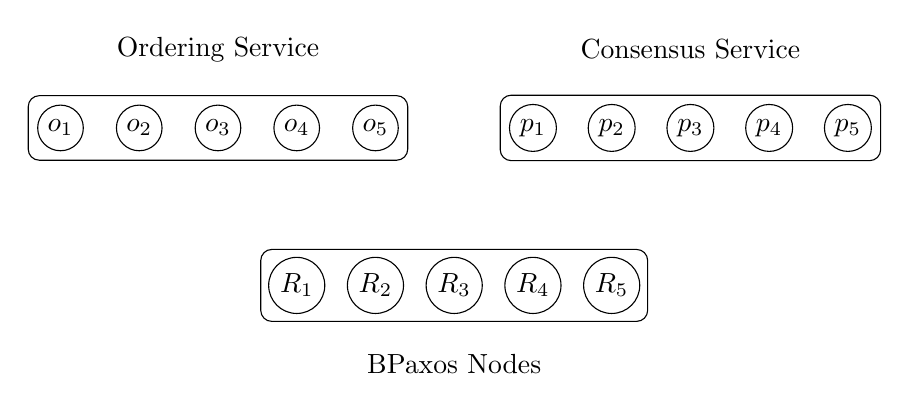
\begin{tikzpicture}
    \tikzstyle{machine}=[draw, circle, inner sep=2pt]

    % Ordering Service
    \node[machine] (o1) at (0, 2) {$o_1$};
    \node[machine] (o2) at (1, 2) {$o_2$};
    \node[machine] (o3) at (2, 2) {$o_3$};
    \node[machine] (o4) at (3, 2) {$o_4$};
    \node[machine] (o5) at (4, 2) {$o_5$};
    \node (os) at (2, 3) {Ordering Service};
    \draw[rounded corners]
      ($(o1.south west) + (-0.2, -0.2)$) rectangle
      ($(o5.north east) + (0.2, 0.2)$);

    % Consensus
    \node[machine] (p1) at (6, 2) {$p_1$};
    \node[machine] (p2) at (7, 2) {$p_2$};
    \node[machine] (p3) at (8, 2) {$p_3$};
    \node[machine] (p4) at (9, 2) {$p_4$};
    \node[machine] (p5) at (10, 2) {$p_5$};
    \node (os) at (8, 3) {Consensus Service};
    \draw[rounded corners]
      ($(p1.south west) + (-0.2, -0.2)$) rectangle
      ($(p5.north east) + (0.2, 0.2)$);

    % BPaxos Nodes
    \node[machine] (b1) at (3, 0) {$R_1$};
    \node[machine] (b2) at (4, 0) {$R_2$};
    \node[machine] (b3) at (5, 0) {$R_3$};
    \node[machine] (b4) at (6, 0) {$R_4$};
    \node[machine] (b5) at (7, 0) {$R_5$};
    \draw[rounded corners]
      ($(b1.south west) + (-0.2, -0.2)$) rectangle
      ($(b5.north east) + (0.2, 0.2)$);
    \node (bpaxos) at (5, -1) {BPaxos Nodes};
  \end{tikzpicture}

  \caption{BPaxos}\figlabel{BPaxos}
\end{figure}
}

\paragraph{Ordering Service}
The ordering service is responsible for computing the dependencies between
conflicting state machine commands. When a BPaxos node $R$ receives a state
machine command $a$ from a client, it chooses a unique instance $R.i$ for $a$.
Then, $R$ sends $(R.i, a)$ to the ordering service. When the ordering service
receives $(R.i, a)$, it replies with a tuple $(R.i, a, \deps{a})$ where
$\deps{a} = \set{I_1, \ldots, I_n}$ is a set of instances called $a$'s
dependencies. The ordering service maintains the following invariant.

\begin{boxedinvariant}\invlabel{OrderingService}
If two conflicting commands $a$ and $b$ in instances $I_a$ and $I_b$ yield
responses $(I_a, a, \deps{a})$ and $(I_b, b, \deps{b})$ from the ordering
service, then either $I_a \in \deps{b}$ or $I_b \in \deps{a}$ (or both). That
is, if two conflicting commands are sent to the ordering service, at least one
is guaranteed to be a dependency of the other.
\end{boxedinvariant}

There are a couple things to note about the ordering service:
\begin{itemize}
  \item
    The ordering service has a precondition that at most one command can be
    sent to the ordering service in any given instance. That is, if a BPaxos
    node sends command $(R.i, a)$ to the ordering service, then no other BPaxos
    node can send $(R.i, b)$ to the ordering service for some other command
    $b$.

  \item
    It's possible that a BPaxos node (or multiple BPaxos nodes) sends the tuple
    $(R.i, a)$ to the ordering service more than once. The ordering service
    does not guarantee that all of the responses to these requests are the
    same.  For example, BPaxos node $R$ may send $(R.1, a)$ to the ordering
    service and get a response $(R.1, a, \set{Q.1, R.2})$. Later, $Q$ might
    send $(R.1, a)$ to the ordering service and get a different response of
    $(R.1, a, \set{Q.2, R.1})$. The ordering service only provides the
    guarantees described by \invref{OrderingService}.
\end{itemize}

\newcommand{\out}{\text{out}}
Implementing a fault tolerant ordering service is straightforward. We employ
$2f + 1$ ordering service nodes $o_{1}, \ldots, o_{2f + 1}$. When a BPaxos node
$R$ sends a command $a$ in instance $R.i$ to the ordering service, it sends the
tuple $(R.i, a)$ to all $2f + 1$ of the ordering service nodes. Every ordering
service node $o_i$ maintains a directed acyclic graph $G_i$. Every vertex of
the graph is labelled with a BPaxos instance and contains a state machine
command. When $o_i$ receives a command $a$ for instance $R.i$ from a Fast
BPaxos node, it performs the following actions:
\begin{enumerate}
  \item
    Let $\out(R.i)$ be the set of outbound edges emanating from the vertex
    labelled $R.i$. If there is already a vertex in $G_i$ labelled $R.i$, then
    $o_i$ returns $(R.i, a, \out(R.i))$ and does nothing else.  Note that the
    ordering service's precondition that most one command can be sent in any
    given instance guarantees that command stored in vertex $R.i$ is $a$.
  \item
    If there does not exist a vertex labelled $R.i$ in $G_i$, then $o_i$
    inserts a vertex into $G_i$ with label $R.i$ and with command $a$. An edge
    is added from instance $R.i$ to instance $Q.j$ for every other instance
    $Q.j$ in the graph that contains a command $b$ that conflicts with $a$.
    $o_i$ then returns the tuple $(R.i, a, \out(R.i))$.
\end{enumerate}

An example of such a graph is given in
\figref{FastPaxosOrderingServiceCartoonBefore}. The same graph is shown
\figref{FastPaxosOrderingServiceCartoonAfter}, except that the command $e$ has
arrived in instance $Q.2$ and conflicts with commands $c$ and $d$.

{\begin{figure}[h]
  \centering

  \begin{subfigure}[b]{0.35\textwidth}
    \begin{tikzpicture}[scale=2.5]
      \node[square] (a) at (0, 1) {$a$};
      \node[square] (b) at (0, 0) {$b$};
      \node[square] (c) at (1, 1) {$c$};
      \node[square] (d) at (1, 0) {$d$};
      \draw[ultra thick, -latex] (c) to (a);
      \draw[ultra thick, -latex] (c) to (b);
      \draw[ultra thick, -latex] (d) to (b);
      \foreach \label/\i in {a/$R.1$, b/$R.2$, c/$Q.1$, d/$S.1$} {%
        \node[above=0in of \label] {\i};
      }
    \end{tikzpicture}
    \caption{}\figlabel{FastPaxosOrderingServiceCartoonBefore}
  \end{subfigure}
  %
  \begin{subfigure}[b]{0.35\textwidth}
    \begin{tikzpicture}[scale=2.5]
      \node[square] (a) at (0, 1) {$a$};
      \node[square] (b) at (0, 0) {$b$};
      \node[square] (c) at (1, 1) {$c$};
      \node[square] (d) at (1, 0) {$d$};
      \node[square] (e) at (2, 0.5) {$e$};
      \draw[ultra thick, -latex] (c) to (a);
      \draw[ultra thick, -latex] (c) to (b);
      \draw[ultra thick, -latex] (d) to (b);
      \draw[ultra thick, -latex] (e) to (c);
      \draw[ultra thick, -latex] (e) to (d);
      \foreach \label/\i in {a/$R.1$, b/$R.2$, c/$Q.1$, d/$S.1$, e/$Q.2$} {%
        \node[above=0in of \label] {\i};
      }
    \end{tikzpicture}
    \caption{}\figlabel{FastPaxosOrderingServiceCartoonAfter}
  \end{subfigure}

  \caption{%
    (left) A directed acyclic graph stored at a Fast BPaxos ordering service
    node. (right) The same graph after the command $e$ arrives in instance
    $Q.2$.
  }\figlabel{FastPaxosOrderingServiceCartoon}
\end{figure}

}

There are a couple of things worth noting about an ordering service node $o_i$
and the corresponding graph $G_i$.
\begin{itemize}
  \item
    $G_i$ is always acyclic.
  \item
    One a gadget $(I_a, a, \out(I_a))$ is inserted into $G_i$, the gadget is
    never modified.
  \item
    The edges in $G_i$ reflect the order in which conflicting commands were
    received by $o_i$. If there is an edge from instance $I_a$ to instance
    $I_b$, then $o_i$ must have received command $b$ in $I_b$ before receiving
    command $a$ in $I_a$.
  \item
    EPaxos and BPaxos both construct a directed cyclic graph of commands that
    are then executed in reverse topological order by strongly component. This
    graph is not the same graph as $G_i$.  $G_i$ is a completely separate graph
    that serves a completely different purpose.
\end{itemize}

When a BPaxos node receives replies $(R.i, a, \deps{a}_{i_1}), \ldots, (R.i, a,
\deps{a}_{i_{f+1}})$ from a quorum $\quorum_a$ of $f + 1$ ordering service
nodes, it takes $(R.i, a, \deps{a}_{i_1} \cup \ldots \cup \deps{a}_{i_{f+1}})$
to be the response from the ordering service. That is, it computes $\deps{a}$
by taking the union of $\deps{a}_i$ from a majority of the ordering service
nodes.

To understand why this ordering service implementation maintains
\invref{OrderingService}, consider conflicting commands $a$ and $b$ in
instances $I_a$ and $I_b$. Assume $a$'s reply $(I_a, a, \deps{a})$ was formed
from a quorum $\quorum_a$ and $b$'s reply $(I_b, b, \deps{b})$ was formed from
a quorum $\quorum_b$. Any two quorums intersect, so $\quorum_a \cap \quorum_b$
is nonempty. Let $o_i$ be an ordering service node in this intersection. $o_i$
either received $a$ or $b$ first. If it received $a$ first, then $G_i$ has a
vertex $I_a$ that contained $a$ when $o_i$ processed command $b$, so $o_i$
includes $I_a$ in $\deps{b}_i$, so $I_a$ is in $\deps{b}$. Symmetrically, if
$o_i$ received $b$ first, then it includes $I_b$ in $\deps{a}$.

\paragraph{Consensus Service}
We assume we have some set $p_1, \ldots, p_n$ of nodes that implement Plain
Jane consensus. A BPaxos node can propose to the consensus service that some
value $v$ be chosen in some instance $I$. The consensus service replies with
the value that has been chosen in instance $I$, which may or may not be $v$
depending on if there are concurrent proposers proposing to instance $i$. The
consensus service guarantees that for every instance $I$, at most one value is
ever chosen in $I$.

We can implement the consensus service with one Paxos instance for every BPaxos
instance, with consensus service nodes playing the role of Paxos acceptors and
the BPaxos nodes playing the role of Paxos proposers. Similar to MultiPaxos, we
can have each BPaxos node $R$ serve as the leader for every Paxos instance
$R.i$. Initially, $R$ runs phase 1 of Paxos for every instance $R.i$, so that
later, $R$ can get a command committed in instance $R.i$ in one round trip to
the consensus service (in the best case).

\paragraph{BPaxos Nodes}
We assume a fixed set $R_1, \ldots, R_{2f+1}$ of $2f + 1$ BPaxos nodes.
%
Clients sends state machine commands to BPaxos nodes to be executed by the
replicated state machine. When a BPaxos node $R$ receives a command $a$, it
sends the command to the ordering service in a previously unused instance $R.i$
and receives a reply $(R.i, a, \deps{a})$. $R$ then proposes the value $(a,
\deps{a})$ to the consensus service in instance $R.i$. The consensus service
then replies with some chosen value $(a', \deps{a'})$ (which is equal to $(a,
\deps{a})$ in the failure-free case). At this point, the gadget $(R.i, a',
\deps{a'})$ is considered chosen in the directed graph of state machine
commands and is eligible for execution. Node $R$ also informs the other BPaxos
nodes that the value $(a', \deps{a'})$ has been chosen.

As noted earlier, the execution of the commands in the directed graph is
identical to that of EPaxos. Committed commands are executed in reverse
topological order, one strongly connected component at a time. Within a
strongly connected component, BPaxos executes commands in an arbitrary but
deterministic order. Unlike with EPaxos, BPaxos does not annotate instances
with sequence numbers. To provide linearizability, when a BPaxos node $R$
receives command $a$ from a client, $R$ does not respond to the client until
the command $a$ has been executed by the replicated state machine. If $R$
returns to the client immediately after $a$ is chosen (as with EPaxos), then
BPaxos provides serializability instead of linearizability.

% Mention that we don't HAVE to no-op.
Note that it's possible that (1) a committed command $a$ depends on an
uncommitted instance $Q.j$, and (2) the BPaxos node $Q$ that manages the
instance $Q.j$ has crashed. If the instance $Q.j$ remains forever uncommitted,
then the command $a$ will never be executed. To avoid this liveness violation,
if any BPaxos node $R$ notices that instance $Q.j$ has been uncommitted for
some time, it can perform one of the following actions:
\begin{enumerate}
  \item
    $R$ can propose to the consensus service that the value $(\noop,
    \emptyset)$ be chosen in instance $Q.j$ where $\noop$ is a command that
    doesn't affect the state machine and doesn't conflict with any other
    command. Note that $R$ does not contact the ordering service here. $R$
    contacts the consensus service directly.

  \item
    $R$ can contact the ordering service and check if any ordering service node
    has recorded a command $b$ in instance $Q.j$. If such a command exists, $R$
    can send the tuple $(Q.j, b)$ to the ordering service, and propose the
    resulting dependencies. If no such command exists, $R$ can propose a
    $\noop$.
\end{enumerate}

\paragraph{Correctness}
BPaxos maintains \invref{GadgetsChosen} trivially because it chooses commands
using consensus. The ordering service maintains \invref{OrderingService}, which
says that the dependencies computed for conflicting commands $a$ and $b$ will
have one in the other (or both). \invref{ConflictingGadgets} says that the
dependencies of conflicting \emph{chosen} commands $a$ and $b$ will have one in
the other (or both). Thus, BPaxos nodes maintain \invref{ConflictingGadgets} by
only proposing dependencies computed by the ordering service. BPaxos nodes also
propose $\noop$'s with empty dependencies, but since $\noop$s do not conflict
with any command, \invref{ConflictingGadgets} is satisfied trivially.

Now, we discuss why \invref{GadgetsChosen} and \invref{ConflictingGadgets}
ensure BPaxos' correctness. Fortunate for us, EPaxos maintains the same two
invariants, so we can leverage EPaxos' proof of correctness. Open up
\cite{moraru2013proof} and head to section 5.6, which contains proofs of
EPaxos' correctness.
\begin{itemize}
  \item
    \textbf{Theorem 1} says that EPaxos satisfies nontriviality. Clearly, so
    does BPaxos.

  \item
    \textbf{Lemma 1} is \invref{GadgetsChosen}. As we saw, BPaxos maintains
    this invariant.

  \item
    \textbf{Theorem 2} follows from Lemma 1.

  \item
    \textbf{Theorem 3} is trivial.

  \item
    \textbf{Theorem 4} states that if two conflicting commands are both
    committed, then they will be executed in the same order by every BPaxos
    node. This follows from \invref{ConflictingGadgets}. If two commands
    conflict, then one will depend on the other or both. If both commands end
    up in the same strongly connected component, they will be executed in the
    same deterministic order. And, if the commands end up in different strongly
    connected components, then one component is guaranteed to be ordered before
    the other, so the two commands are executed in reverse topological order.
\end{itemize}

}
{\section{Simple BPaxos}
In this section, we introduce \defword{Simple BPaxos}, a BPaxos protocol that
is designed to be as simple as possible.
%
Simple BPaxos consists of three logical components: a set of Simple BPaxos
nodes, a dependency service, and a consensus service. The dependency service
helps provide \invref{ConflictInvariant}, the consensus service helps provide
\invref{ConsensusInvariant}, and the Simple BPaxos nodes glue the two together.
We explain each of these three components in turn. Throughout our discussion,
we assume at most $f$ processes can fail.

\subsection{Simple BPaxos Nodes}
We assume a fixed set $b_1, \ldots, b_{f+1}$ of $f + 1$ Simple BPaxos nodes.
Each Simple BPaxos node $b_i$ is a state machine replica and is responsible for
learning a partial instance graph and processing commands as described in
\secref{BipartisanPaxos}.
%
Clients sends state machine commands to BPaxos nodes to be executed by the
replicated state machine. When a BPaxos node $b_i$ receives a command $x$, it
selects a globally unique instance $I$ for the command and sends the tuple $(I,
x)$ to the dependency service. The dependency service replies with a tuple $(I,
x, \deps{I})$ where $\deps{I}$ is a set of instances.
%
$b_i$ then proposes the value $(x, \deps{I})$ to the consensus service in
instance $I$, and the consensus service replies with some chosen value $(x',
\deps{I}')$ (which is equal to $(x, \deps{I})$ in the failure-free case). At
this point, the command $x'$ with dependencies $\deps{I}'$ is chosen in instance
$I$ and is added to $b_i$'s partial instance graph. $b_i$ also informs the
other Simple BPaxos nodes that the command $x'$ with dependencies $\deps{I}'$
have been chosen in instance $I$.

\subsection{Dependency Service}
Upon receiving a tuple $(I, x)$ from a Simple BPaxos node, the dependency
service replies with a tuple $(I, x, \deps{I})$ with the following guarantee.

\begin{invariant}\invlabel{DependencyService}
If two conflicting commands $x$ and $y$ in instances $I_x$ and $I_y$ yield
responses $(I_x, x, \deps{I_x})$ and $(I_y, y, \deps{x})$ from the dependency
service, then either $I_x \in \deps{I_y}$ or $I_y \in \deps{I_x}$ (or both).
\end{invariant}

There are a couple things to note about the dependency service.
%
First, the dependency service has a precondition that at most one command can
be sent to the dependency service in any given instance. That is, if a Simple
BPaxos node sends the tuple $(I, x)$ to the dependency service, then no other
Simple BPaxos node can send the tuple $(I, y)$ to the dependency service for
some other command $y$.
%
Second, the dependency service may receive the tuple $(I, x)$ more than once.
The dependency service does not guarantee that all of its responses will be the
same. For example, Simple BPaxos node $b_i$ may send $(I, x)$ to the dependency
service and get a response $(I, x, \set{I_1, I_2})$. Later, $b_j$ might send
$(I, x)$ to the dependency service and get a different response of $(I, x,
\set{I_2, I_3})$. Note that even though the dependency service may produce
different responses for the same request, the dependency service maintains
\invref{DependencyService} for every possible pair of dependency service
responses.

\newcommand{\out}[1]{\text{out}(#1)}
We now describe how to implement the dependency service. We employ $2f + 1$
dependency service nodes $d_{1}, \ldots, d_{2f + 1}$. When a Simple BPaxos node
$b_i$ sends the tuple $(I, x)$ to the dependency service, it sends the tuple to
all $2f + 1$ of the dependency service nodes. Every dependency service node
$d_i$ maintains a conflict graph $G_i$ with instances as vertices. When $d_i$
receives a command $x$ for instance $I$ from a Simple BPaxos node, it performs
the following actions.
%
If $G_i$ already contains vertex $I$, then $d_i$ returns the tuple $(I, x,
\out{I})$ where $\out{I}$ is the set of instances with an inbound edge from
$I$.
%
Otherwise, $d_i$ inserts vertex $I$ into $G_i$ with label $x$ and with edges to
every other instance $I'$ in $G_i$ that is labelled with a command that
conflicts with $x$. Then, $d_i$ returns $(I, x, \out{I})$.
%
When a Simple BPaxos node $b_j$ receives replies $(I, x, \deps{I}_{i_1}),
\ldots, (I, x, \deps{I}_{i_{f+1}})$ from a quorum $\Quorum$ of $f + 1$
dependency service nodes $d_{i_1}, \ldots, d_{i_{f+1}}$, it takes $(I, x,
\deps{I}_{i_1} \cup \ldots \cup \deps{x}_{i_{f+1}})$ to be the response from
the dependency service. That is, $b_j$ computes $\deps{I}$ by taking the union
of dependencies from a majority of the dependency service nodes.

To understand why this dependency service implementation maintains
\invref{DependencyService}, consider conflicting commands $x$ and $y$ in
instances $I_x$ and $I_y$. Assume $x$'s reply $(I_x, x, \deps{I_x})$ was formed
from a quorum $\Quorum_x$ and $y$'s reply $(I_y, y, \deps{y})$ was formed from
a quorum $\Quorum_y$. Any two quorums intersect, so $\Quorum_x \cap \Quorum_y$
is nonempty. Let $d_i$ be a dependency service node in this intersection. $d_i$
either received $(I_x, x)$ or $(I_y, y)$ first. If it received $I_x$ first,
then $I_y$ has an edge to $I_x$ in $G_i$, so $I_x \in \deps{I_y}$.
Symmetrically, if it received $I_y$ first, then $I_x$ has an edge to $I_y$ in
$G_i$, so $I_y \in \deps{I_x}$.

\subsection{Consensus Service}
We assume a consensus service that implements consensus for every instance $I$.
A Simple BPaxos node can propose to the consensus service that some value $v$
be chosen in some instance $I$. The consensus service replies with the value
that has been chosen in instance $I$, which may or may not be $v$. The
consensus service guarantees that for every instance $I$, at most one value is
ever chosen in $I$. The consensus service can be implemented with any consensus
protocol (e.g., Paxos).

\subsection{Recovery}
Note that it's possible that a command $x$ chosen in instance $I$ depends on an
uncommitted instance $I'$. If instance $I'$ remains forever unchosen, then the
command $x$ will never be executed. To avoid this liveness violation, if any
Simple BPaxos node $b_i$ notices that instance $I'$ has been unchosen for some
time, $b_i$ can propose to the consensus service that the command $\noop$ be
chosen in instance $I'$ with no dependencies. $\noop$ is a distinguished
command that does not affect the state machine and does not conflict with any
other command.
%
Alternatively, $b_i$ can contact the dependency service and check if any
dependency service node has recorded a command $y$ in instance $I'$. If such a
command exists, $b_i$ can send the tuple $(I, y)$ to the dependency service,
and propose the resulting dependencies. If no such command exists, $b_i$ can
propose a $\noop$.

\subsection{Correctness}
Simple BPaxos maintains \invref{ConsensusInvariant} by leveraging the consensus
service. Simple BPaxos maintains \invref{ConflictInvariant} by leveraging the
dependency service. More carefully, if any two conflicting commands $x$ and $y$
are chosen in instances $I_x$ and $I_y$ with dependencies $\deps{I_x}$ and
$\deps{I_y}$, then the tuples $(I_x, x, \deps{I_x})$ and $(I_y, y, \deps{I_y})$
must have been returned by the dependency service because Simple BPaxos nodes
only propose dependencies computed by the ordering service (and $\noop$s, which
we touch on momentarily). Thus, \invref{ConflictInvariant} follows immediately
from \invref{DependencyService}. Note that proposing $\noop{}$s does not
affect \invref{ConflictInvariant} because $\noop$s do not conflict with any
other command, so \invref{ConflictInvariant} holds vacuously.

\subsection{Discussion}
\TODO[mwhittaker]{Highlight the modularity of the protocol.}
\TODO[mwhittaker]{Describe that clients can initiate the protocol, and don't have to send to Simple BPaxos nodes.}
}
{\section{Fast Paxos}\seclabel{FastPaxos}
{\newcommand{\nullbot}{\textsf{null}}

\begin{algorithm}[ht]
  \caption{Fast Paxos Proposer}%
  \algolabel{FastPaxosProposer}
  \begin{algorithmic}[1]
    \GlobalState a value $v$, initially \nullbot{}
    \GlobalState a round $i$, initially $-1$

    \Upon{%
      receiving \msg{Phase2B}{0, v'} from $f + \maj{f+1}$

      \hspace{0.06in}acceptors as the proposer of round $0$ with $i=0$
    }\linelabel{Proposer1}
      \If{every value of $v'$ is the same}
        \State $v'$ is chosen, notify the learners \linelabel{Proposer2}
      \Else{} \linelabel{CoordinatedRecovery1}
        \State $i \gets 1$
        \State proceed to \lineref{computek} viewing every \msg{Phase2B}{0, v'}

        \hspace{0.13in}as a \msg{Phase1B}{1, 0, v'}
      \EndIf \linelabel{CoordinatedRecovery2}
    \EndUpon

    \Upon{recovery}\linelabel{ProposerRecovery1}
      \State $i \gets$ next largest round owned by this proposer
      % Addresses Reviewer 3.
      %
      % > I am unsure why at line 21 of Algorithm 1, the propose is sending to at
      % > least $f+1$ acceptors instead of all acceptors. As $f$ of the acceptors
      % > may crash, so sending to all acceptors in important.
      \State send \msg{Phase1A}{i} to \markrevisions{the acceptors}
    \EndUpon\linelabel{ProposerRecovery2}

    \Upon{receiving \msg{Phase1B}{i, vr, vv} from $f+1$ acceptors}
      \State $k \gets$ the largest $vr$ in any \msg{Phase1B}{i, vr, vv}\linelabel{computek}
      \If{$k = -1$}\linelabel{kn1}
        \State $v \gets$ an arbitrary value
      \ElsIf{$k > 0$}\linelabel{kg0}
        \State $v \gets$ the corresponding $vv$ in round $k$
      \ElsIf{$k = 0$}\linelabel{ke0}
      \If{there are $\maj{f + 1}$ \msg{Phase1B}{i, 0, v'}

          \hspace{0.22in} messages for some value $v'$}\linelabel{majority}
          \State $v \gets$ $v'$
        \Else{}\linelabel{nomajority}
          \State $v \gets$ an arbitrary value
        \EndIf
      \EndIf
      % Addresses Reviewer 3.
      %
      % > I am unsure why at line 21 of Algorithm 1, the propose is sending to at
      % > least $f+1$ acceptors instead of all acceptors. As $f$ of the acceptors
      % > may crash, so sending to all acceptors in important.
      \State send \msg{Phase2A}{i, v} to \markrevisions{the acceptors}
    \EndUpon

    \Upon{receiving \msg{Phase2B}{i} from $f+1$ acceptors}
      \State $v$ is chosen, notify the learners
    \EndUpon
  \end{algorithmic}
\end{algorithm}
}
{\newcommand{\nullbot}{\textsf{null}}

\begin{algorithm}[ht]
  \caption{Fast Paxos Acceptor}%
  \algolabel{FastPaxosAcceptor}
  \begin{algorithmic}[1]
    \GlobalState the largest seen round $r$, initially $-1$
    \GlobalState the largest round $vr$ voted in, initially $-1$
    \GlobalState the value $vv$ voted for in round $vr$, initially \nullbot{}

    \Upon{receiving command $x$ from client} \linelabel{Acceptor1}
      \If{$r = -1$}
        \State $r, vr, vv \gets 0, 0, x$
        \State send \msg{Phase2b}{0, x} to proposer of round $0$
      \EndIf
    \EndUpon{} \linelabel{Acceptor2}

    \Upon{receiving \msg{Phase1A}{i} from $p$ with $i > r$}\linelabel{AcceptorPhase11}
      \State $r \gets i$
      \State send \msg{Phase1B}{i, vr, vv} to $p$
    \EndUpon \linelabel{AcceptorPhase12}

    \Upon{receiving \msg{Phase2A}{i, x} from $p$ with $i \geq r$}
      \State $r, vr, vv \gets i, i, x$
      \State send \msg{Phase2B}{i} to $p$
    \EndUpon
  \end{algorithmic}
\end{algorithm}
}
{\section{Fast Paxos}\seclabel{FastPaxos}
{\newcommand{\nullbot}{\textsf{null}}

\begin{algorithm}[ht]
  \caption{Fast Paxos Proposer}%
  \algolabel{FastPaxosProposer}
  \begin{algorithmic}[1]
    \GlobalState a value $v$, initially \nullbot{}
    \GlobalState a round $i$, initially $-1$

    \Upon{%
      receiving \msg{Phase2B}{0, v'} from $f + \maj{f+1}$

      \hspace{0.06in}acceptors as the proposer of round $0$ with $i=0$
    }\linelabel{Proposer1}
      \If{every value of $v'$ is the same}
        \State $v'$ is chosen, notify the learners \linelabel{Proposer2}
      \Else{} \linelabel{CoordinatedRecovery1}
        \State $i \gets 1$
        \State proceed to \lineref{computek} viewing every \msg{Phase2B}{0, v'}

        \hspace{0.13in}as a \msg{Phase1B}{1, 0, v'}
      \EndIf \linelabel{CoordinatedRecovery2}
    \EndUpon

    \Upon{recovery}\linelabel{ProposerRecovery1}
      \State $i \gets$ next largest round owned by this proposer
      % Addresses Reviewer 3.
      %
      % > I am unsure why at line 21 of Algorithm 1, the propose is sending to at
      % > least $f+1$ acceptors instead of all acceptors. As $f$ of the acceptors
      % > may crash, so sending to all acceptors in important.
      \State send \msg{Phase1A}{i} to \markrevisions{the acceptors}
    \EndUpon\linelabel{ProposerRecovery2}

    \Upon{receiving \msg{Phase1B}{i, vr, vv} from $f+1$ acceptors}
      \State $k \gets$ the largest $vr$ in any \msg{Phase1B}{i, vr, vv}\linelabel{computek}
      \If{$k = -1$}\linelabel{kn1}
        \State $v \gets$ an arbitrary value
      \ElsIf{$k > 0$}\linelabel{kg0}
        \State $v \gets$ the corresponding $vv$ in round $k$
      \ElsIf{$k = 0$}\linelabel{ke0}
      \If{there are $\maj{f + 1}$ \msg{Phase1B}{i, 0, v'}

          \hspace{0.22in} messages for some value $v'$}\linelabel{majority}
          \State $v \gets$ $v'$
        \Else{}\linelabel{nomajority}
          \State $v \gets$ an arbitrary value
        \EndIf
      \EndIf
      % Addresses Reviewer 3.
      %
      % > I am unsure why at line 21 of Algorithm 1, the propose is sending to at
      % > least $f+1$ acceptors instead of all acceptors. As $f$ of the acceptors
      % > may crash, so sending to all acceptors in important.
      \State send \msg{Phase2A}{i, v} to \markrevisions{the acceptors}
    \EndUpon

    \Upon{receiving \msg{Phase2B}{i} from $f+1$ acceptors}
      \State $v$ is chosen, notify the learners
    \EndUpon
  \end{algorithmic}
\end{algorithm}
}
{\newcommand{\nullbot}{\textsf{null}}

\begin{algorithm}[ht]
  \caption{Fast Paxos Acceptor}%
  \algolabel{FastPaxosAcceptor}
  \begin{algorithmic}[1]
    \GlobalState the largest seen round $r$, initially $-1$
    \GlobalState the largest round $vr$ voted in, initially $-1$
    \GlobalState the value $vv$ voted for in round $vr$, initially \nullbot{}

    \Upon{receiving command $x$ from client} \linelabel{Acceptor1}
      \If{$r = -1$}
        \State $r, vr, vv \gets 0, 0, x$
        \State send \msg{Phase2b}{0, x} to proposer of round $0$
      \EndIf
    \EndUpon{} \linelabel{Acceptor2}

    \Upon{receiving \msg{Phase1A}{i} from $p$ with $i > r$}\linelabel{AcceptorPhase11}
      \State $r \gets i$
      \State send \msg{Phase1B}{i, vr, vv} to $p$
    \EndUpon \linelabel{AcceptorPhase12}

    \Upon{receiving \msg{Phase2A}{i, x} from $p$ with $i \geq r$}
      \State $r, vr, vv \gets i, i, x$
      \State send \msg{Phase2B}{i} to $p$
    \EndUpon
  \end{algorithmic}
\end{algorithm}
}
{\section{Fast Paxos}\seclabel{FastPaxos}
{\input{figures/fast_paxos_proposer.tex}}
{\input{figures/fast_paxos_acceptor.tex}}
{\input{figures/fast_paxos.tex}}

Simple \BPaxos{} is designed to be easy to understand, but as shown in
\figref{SimpleBPaxosExample}, it takes seven network delays (in the best case)
between when a client proposes a command $x$ and when a client receives the
result of executing $x$. Call this duration of time the \defword{commit time}.
Generalized multi-leader protocols like EPaxos, Caesar, and Atlas all achieve a
commit time of only four network delays. They do so by leveraging Fast
Paxos~\cite{lamport2006fast}.

Fast Paxos is a Paxos variant that allows clients to propose values directly to
the acceptors without having to initially contact a proposer. Fast Paxos is an
optimistic protocol. If all of the acceptors happen to receive the same command
from the clients, then Fast Paxos has a commit time of only three network
delays. This is called the fast path. However, if multiple clients concurrently
propose different commands, and not all of the acceptors receive the same
command, then the protocol reverts to a slow path and introduces two additional
network delays to the commit time.  In this section, we review a slightly
simplified version of Fast Paxos.

Like Paxos, a Fast Paxos deployment consists of some number of clients, $f+1$
proposers, and $2f+1$ acceptors. We also include a set of $f+1$ learners. These
nodes are notified of the value chosen by Fast Paxos. A Fast Paxos deployment
is illustrated in \figref{FastPaxos}. Proposer and acceptor pseudocode
are given in \algoref{FastPaxosProposer} and \algoref{FastPaxosAcceptor}.

Like Paxos, Fast Paxos is divided into a number of integer valued rounds.  The
key difference is that round 0 of Fast Paxos is a special ``fast round.'' A
client can propose a value directly to an acceptor in round 0 without having to
contact a proposer first. The normal case execution of Fast Paxos is
illustrated in \figref{FastPaxos1}. The execution proceeds as follows:

\begin{itemize}
  \item \textbf{(1)}
    When a client wants to propose a value $v$, it sends $v$ to all of the
    acceptors.

  \item \textbf{(2)}
    When an acceptor receives a value $v$ from a client, the acceptor ignores
    $v$ if it has already received a message in some round $i \geq 0$.
    Otherwise, it votes for $v$ by updating its state and sending a
    \msg{Phase2B}{0, v} message to the proposer that leads round $0$. This is
    shown in \algoref{FastPaxosAcceptor} \lineref{Acceptor1} --
    \lineref{Acceptor2}.

  \item \textbf{(3)}
    Let $\maj{n}$ be a majority of $n$. $\maj{n} = \frac{n}{2} + 1$ if $n$ is
    even, and $\maj{n} = \ceil{n/2}$ if $n$ is odd. If the proposer that leads
    round $0$ receives \msg{Phase2B}{0, $v'$} messages from $f + \maj{f+1}$
    acceptors for the same value $v'$, then $v'$ is chosen, and the proposer
    notifies the learners. This is shown in \algoref{FastPaxosProposer}
    \lineref{Proposer1} -- \lineref{Proposer2}. We consider what happens when
    not every value is the same momentarily.
\end{itemize}

Note that in Paxos, a value is chosen when $f+1$ acceptors vote for it in some
round $i$. In round $0$ of Fast Paxos, a value is chosen when $f + \maj{f+1}$
acceptors vote for it. The larger number of required votes is needed to ensure
the safety of recovery, which we now describe.
%
Let $p$ be the proposer leading round $0$. Recovery is the process by which a
proposer other than $p$ gets a value chosen. For example, if $p$ fails, some
other proposer must take over and get a value chosen. Recovery is illustrated
in \figref{FastPaxos2}.

\begin{itemize}
  \item \textbf{(1) and (2)}
    A recovering proposer performs Phase 1 of Paxos with at least $f+1$
    acceptors in some round $i > 0$. This is shown in
    \algoref{FastPaxosProposer} \lineref{ProposerRecovery1} --
    \lineref{ProposerRecovery2} and \algoref{FastPaxosAcceptor}
    \lineref{AcceptorPhase11} -- \lineref{AcceptorPhase12}.

  \item \textbf{(3) and (4)}
    The recovering proposer receives \msg{Phase1B}{i, vr, vv} messages from
    $f+1$ acceptors. Call this quorum of acceptors $A$. The proposer computes
    $k$ as the largest received $vr$ (\lineref{computek}). This is the largest
    round in which any acceptor in $A$ has voted. If $k = -1$ (\lineref{kn1}),
    then none of the acceptors have voted in any round less than $i$, so the
    proposer is free to propose an arbitrary value. This is the same as in
    Paxos. If $k > 0$ (\lineref{kg0}), then the proposer must propose the value
    $vv$ proposed in round $k$. Again, this is the same as in Paxos. $vv$ may
    have been chosen in round $k$, so the proposer is forced to propose it as
    well. If $k = 0$ (\lineref{ke0}), then there are two cases to consider.

    First, if $\maj{f+1}$ of the acceptors in $A$ have all voted for some value
    $v'$ in round $0$, then it's possible that $v'$ was chosen in round $0$
    (\lineref{majority}). Specifically, if all $f$ of the acceptors not in $A$
    voted for $v'$ in round $0$, then along with the $\maj{f+1}$ of acceptors in
    $A$ who also voted for $v'$ in round $0$, there is a quorum of $f +
    \maj{f+1}$ acceptors who voted for $v'$ in round $0$. In this case, the
    proposer must propose $v'$ as well since it might have been chosen. Second,
    if there does not exist $\maj{f+1}$ votes for any value $v'$, then the
    proposer concludes that no value was chosen or every will be chosen in
    round $0$, so it is free to propose an arbitrary value
    (\lineref{nomajority}).

    Note that a value must receive at least $f + \maj{f+1}$ votes in round $0$
    to be chosen. If this number were any smaller, it would be possible for a
    recovering proposer to find two distinct values $v'$ and $v''$ that
    \emph{both} could have been chosen in round $0$. In this case, the proposer
    cannot make progress. It cannot propose $v'$ because $v''$ might have been
    chosen, and it cannot propose $v''$ because $v'$ might have been chosen

    Once the recovering proposer determines which value to propose, it gets the
    value chosen with the acceptors using the normal Phase 2 of Paxos.

  \item \textbf{(5)}
    The proposer notifies the learners of the chosen value.
\end{itemize}

Finally, we consider what happens when the proposer of round $0$ receives $f +
\maj{f+1}$ \msgfont{Phase1B} messages from the acceptors, but without all of
them containing the same value $v'$. Naively, the proposer could simply
perform a recovery, executing both phases of Paxos is some round $i > 0$.
However, if we assign rounds to proposers in such a way that the proposer of
round $0$ is also the proposer of round $1$, then we can take advantage of an
optimization called \defword{coordinated recovery}. This is illustrated in
\figref{FastPaxos3} and proceeds as follows:

\begin{itemize}
  \item \textbf{(1)}
    Multiple clients send distinct commands directly to the acceptors.

  \item \textbf{(2)}
    The acceptors receive and vote for the commands and send \msgfont{Phase2B}
    messages to the leader of round $0$. However, not every acceptor receives
    the same value first, so not all the acceptors vote for the same value.

  \item \textbf{(3) and (4)}
    The proposer receives \msgfont{Phase2B} messages from $f+\maj{f+1}$
    acceptors, but the acceptors have not all voted for the same value. At this
    point, the proposer could naively perform a recovery in round $1$ by
    executing Phase 1 and then Phase 2 of Paxos. But, executing Phase 1 in
    round $1$ is redundant, since the \msgfont{Phase2B} messages in round $0$
    contain exactly the same information as the \msgfont{Phase1B} messages in
    round $1$. Specifically, the proposer can view every \msg{Phase2B}{0, v'}
    message as a proxy for a \msg{Phase1B}{1, 0, v'} message. Thus, the proposer
    instead jumps immediately to Phase 2 in round $1$ to get a value chosen
    (\lineref{CoordinatedRecovery1} -- \lineref{CoordinatedRecovery2}).

  \item \textbf{(5)}
    Finally, the proposer notifies the learners of the chosen value.
\end{itemize}
}

Simple \BPaxos{} is designed to be easy to understand, but as shown in
\figref{SimpleBPaxosExample}, it takes seven network delays (in the best case)
between when a client proposes a command $x$ and when a client receives the
result of executing $x$. Call this duration of time the \defword{commit time}.
Generalized multi-leader protocols like EPaxos, Caesar, and Atlas all achieve a
commit time of only four network delays. They do so by leveraging Fast
Paxos~\cite{lamport2006fast}.

Fast Paxos is a Paxos variant that allows clients to propose values directly to
the acceptors without having to initially contact a proposer. Fast Paxos is an
optimistic protocol. If all of the acceptors happen to receive the same command
from the clients, then Fast Paxos has a commit time of only three network
delays. This is called the fast path. However, if multiple clients concurrently
propose different commands, and not all of the acceptors receive the same
command, then the protocol reverts to a slow path and introduces two additional
network delays to the commit time.  In this section, we review a slightly
simplified version of Fast Paxos.

Like Paxos, a Fast Paxos deployment consists of some number of clients, $f+1$
proposers, and $2f+1$ acceptors. We also include a set of $f+1$ learners. These
nodes are notified of the value chosen by Fast Paxos. A Fast Paxos deployment
is illustrated in \figref{FastPaxos}. Proposer and acceptor pseudocode
are given in \algoref{FastPaxosProposer} and \algoref{FastPaxosAcceptor}.

Like Paxos, Fast Paxos is divided into a number of integer valued rounds.  The
key difference is that round 0 of Fast Paxos is a special ``fast round.'' A
client can propose a value directly to an acceptor in round 0 without having to
contact a proposer first. The normal case execution of Fast Paxos is
illustrated in \figref{FastPaxos1}. The execution proceeds as follows:

\begin{itemize}
  \item \textbf{(1)}
    When a client wants to propose a value $v$, it sends $v$ to all of the
    acceptors.

  \item \textbf{(2)}
    When an acceptor receives a value $v$ from a client, the acceptor ignores
    $v$ if it has already received a message in some round $i \geq 0$.
    Otherwise, it votes for $v$ by updating its state and sending a
    \msg{Phase2B}{0, v} message to the proposer that leads round $0$. This is
    shown in \algoref{FastPaxosAcceptor} \lineref{Acceptor1} --
    \lineref{Acceptor2}.

  \item \textbf{(3)}
    Let $\maj{n}$ be a majority of $n$. $\maj{n} = \frac{n}{2} + 1$ if $n$ is
    even, and $\maj{n} = \ceil{n/2}$ if $n$ is odd. If the proposer that leads
    round $0$ receives \msg{Phase2B}{0, $v'$} messages from $f + \maj{f+1}$
    acceptors for the same value $v'$, then $v'$ is chosen, and the proposer
    notifies the learners. This is shown in \algoref{FastPaxosProposer}
    \lineref{Proposer1} -- \lineref{Proposer2}. We consider what happens when
    not every value is the same momentarily.
\end{itemize}

Note that in Paxos, a value is chosen when $f+1$ acceptors vote for it in some
round $i$. In round $0$ of Fast Paxos, a value is chosen when $f + \maj{f+1}$
acceptors vote for it. The larger number of required votes is needed to ensure
the safety of recovery, which we now describe.
%
Let $p$ be the proposer leading round $0$. Recovery is the process by which a
proposer other than $p$ gets a value chosen. For example, if $p$ fails, some
other proposer must take over and get a value chosen. Recovery is illustrated
in \figref{FastPaxos2}.

\begin{itemize}
  \item \textbf{(1) and (2)}
    A recovering proposer performs Phase 1 of Paxos with at least $f+1$
    acceptors in some round $i > 0$. This is shown in
    \algoref{FastPaxosProposer} \lineref{ProposerRecovery1} --
    \lineref{ProposerRecovery2} and \algoref{FastPaxosAcceptor}
    \lineref{AcceptorPhase11} -- \lineref{AcceptorPhase12}.

  \item \textbf{(3) and (4)}
    The recovering proposer receives \msg{Phase1B}{i, vr, vv} messages from
    $f+1$ acceptors. Call this quorum of acceptors $A$. The proposer computes
    $k$ as the largest received $vr$ (\lineref{computek}). This is the largest
    round in which any acceptor in $A$ has voted. If $k = -1$ (\lineref{kn1}),
    then none of the acceptors have voted in any round less than $i$, so the
    proposer is free to propose an arbitrary value. This is the same as in
    Paxos. If $k > 0$ (\lineref{kg0}), then the proposer must propose the value
    $vv$ proposed in round $k$. Again, this is the same as in Paxos. $vv$ may
    have been chosen in round $k$, so the proposer is forced to propose it as
    well. If $k = 0$ (\lineref{ke0}), then there are two cases to consider.

    First, if $\maj{f+1}$ of the acceptors in $A$ have all voted for some value
    $v'$ in round $0$, then it's possible that $v'$ was chosen in round $0$
    (\lineref{majority}). Specifically, if all $f$ of the acceptors not in $A$
    voted for $v'$ in round $0$, then along with the $\maj{f+1}$ of acceptors in
    $A$ who also voted for $v'$ in round $0$, there is a quorum of $f +
    \maj{f+1}$ acceptors who voted for $v'$ in round $0$. In this case, the
    proposer must propose $v'$ as well since it might have been chosen. Second,
    if there does not exist $\maj{f+1}$ votes for any value $v'$, then the
    proposer concludes that no value was chosen or every will be chosen in
    round $0$, so it is free to propose an arbitrary value
    (\lineref{nomajority}).

    Note that a value must receive at least $f + \maj{f+1}$ votes in round $0$
    to be chosen. If this number were any smaller, it would be possible for a
    recovering proposer to find two distinct values $v'$ and $v''$ that
    \emph{both} could have been chosen in round $0$. In this case, the proposer
    cannot make progress. It cannot propose $v'$ because $v''$ might have been
    chosen, and it cannot propose $v''$ because $v'$ might have been chosen

    Once the recovering proposer determines which value to propose, it gets the
    value chosen with the acceptors using the normal Phase 2 of Paxos.

  \item \textbf{(5)}
    The proposer notifies the learners of the chosen value.
\end{itemize}

Finally, we consider what happens when the proposer of round $0$ receives $f +
\maj{f+1}$ \msgfont{Phase1B} messages from the acceptors, but without all of
them containing the same value $v'$. Naively, the proposer could simply
perform a recovery, executing both phases of Paxos is some round $i > 0$.
However, if we assign rounds to proposers in such a way that the proposer of
round $0$ is also the proposer of round $1$, then we can take advantage of an
optimization called \defword{coordinated recovery}. This is illustrated in
\figref{FastPaxos3} and proceeds as follows:

\begin{itemize}
  \item \textbf{(1)}
    Multiple clients send distinct commands directly to the acceptors.

  \item \textbf{(2)}
    The acceptors receive and vote for the commands and send \msgfont{Phase2B}
    messages to the leader of round $0$. However, not every acceptor receives
    the same value first, so not all the acceptors vote for the same value.

  \item \textbf{(3) and (4)}
    The proposer receives \msgfont{Phase2B} messages from $f+\maj{f+1}$
    acceptors, but the acceptors have not all voted for the same value. At this
    point, the proposer could naively perform a recovery in round $1$ by
    executing Phase 1 and then Phase 2 of Paxos. But, executing Phase 1 in
    round $1$ is redundant, since the \msgfont{Phase2B} messages in round $0$
    contain exactly the same information as the \msgfont{Phase1B} messages in
    round $1$. Specifically, the proposer can view every \msg{Phase2B}{0, v'}
    message as a proxy for a \msg{Phase1B}{1, 0, v'} message. Thus, the proposer
    instead jumps immediately to Phase 2 in round $1$ to get a value chosen
    (\lineref{CoordinatedRecovery1} -- \lineref{CoordinatedRecovery2}).

  \item \textbf{(5)}
    Finally, the proposer notifies the learners of the chosen value.
\end{itemize}
}

Simple \BPaxos{} is designed to be easy to understand, but as shown in
\figref{SimpleBPaxosExample}, it takes seven network delays (in the best case)
between when a client proposes a command $x$ and when a client receives the
result of executing $x$. Call this duration of time the \defword{commit time}.
Generalized multi-leader protocols like EPaxos, Caesar, and Atlas all achieve a
commit time of only four network delays. They do so by leveraging Fast
Paxos~\cite{lamport2006fast}.

Fast Paxos is a Paxos variant that allows clients to propose values directly to
the acceptors without having to initially contact a proposer. Fast Paxos is an
optimistic protocol. If all of the acceptors happen to receive the same command
from the clients, then Fast Paxos has a commit time of only three network
delays. This is called the fast path. However, if multiple clients concurrently
propose different commands, and not all of the acceptors receive the same
command, then the protocol reverts to a slow path and introduces two additional
network delays to the commit time.  In this section, we review a slightly
simplified version of Fast Paxos.

Like Paxos, a Fast Paxos deployment consists of some number of clients, $f+1$
proposers, and $2f+1$ acceptors. We also include a set of $f+1$ learners. These
nodes are notified of the value chosen by Fast Paxos. A Fast Paxos deployment
is illustrated in \figref{FastPaxos}. Proposer and acceptor pseudocode
are given in \algoref{FastPaxosProposer} and \algoref{FastPaxosAcceptor}.

Like Paxos, Fast Paxos is divided into a number of integer valued rounds.  The
key difference is that round 0 of Fast Paxos is a special ``fast round.'' A
client can propose a value directly to an acceptor in round 0 without having to
contact a proposer first. The normal case execution of Fast Paxos is
illustrated in \figref{FastPaxos1}. The execution proceeds as follows:

\begin{itemize}
  \item \textbf{(1)}
    When a client wants to propose a value $v$, it sends $v$ to all of the
    acceptors.

  \item \textbf{(2)}
    When an acceptor receives a value $v$ from a client, the acceptor ignores
    $v$ if it has already received a message in some round $i \geq 0$.
    Otherwise, it votes for $v$ by updating its state and sending a
    \msg{Phase2B}{0, v} message to the proposer that leads round $0$. This is
    shown in \algoref{FastPaxosAcceptor} \lineref{Acceptor1} --
    \lineref{Acceptor2}.

  \item \textbf{(3)}
    Let $\maj{n}$ be a majority of $n$. $\maj{n} = \frac{n}{2} + 1$ if $n$ is
    even, and $\maj{n} = \ceil{n/2}$ if $n$ is odd. If the proposer that leads
    round $0$ receives \msg{Phase2B}{0, $v'$} messages from $f + \maj{f+1}$
    acceptors for the same value $v'$, then $v'$ is chosen, and the proposer
    notifies the learners. This is shown in \algoref{FastPaxosProposer}
    \lineref{Proposer1} -- \lineref{Proposer2}. We consider what happens when
    not every value is the same momentarily.
\end{itemize}

Note that in Paxos, a value is chosen when $f+1$ acceptors vote for it in some
round $i$. In round $0$ of Fast Paxos, a value is chosen when $f + \maj{f+1}$
acceptors vote for it. The larger number of required votes is needed to ensure
the safety of recovery, which we now describe.
%
Let $p$ be the proposer leading round $0$. Recovery is the process by which a
proposer other than $p$ gets a value chosen. For example, if $p$ fails, some
other proposer must take over and get a value chosen. Recovery is illustrated
in \figref{FastPaxos2}.

\begin{itemize}
  \item \textbf{(1) and (2)}
    A recovering proposer performs Phase 1 of Paxos with at least $f+1$
    acceptors in some round $i > 0$. This is shown in
    \algoref{FastPaxosProposer} \lineref{ProposerRecovery1} --
    \lineref{ProposerRecovery2} and \algoref{FastPaxosAcceptor}
    \lineref{AcceptorPhase11} -- \lineref{AcceptorPhase12}.

  \item \textbf{(3) and (4)}
    The recovering proposer receives \msg{Phase1B}{i, vr, vv} messages from
    $f+1$ acceptors. Call this quorum of acceptors $A$. The proposer computes
    $k$ as the largest received $vr$ (\lineref{computek}). This is the largest
    round in which any acceptor in $A$ has voted. If $k = -1$ (\lineref{kn1}),
    then none of the acceptors have voted in any round less than $i$, so the
    proposer is free to propose an arbitrary value. This is the same as in
    Paxos. If $k > 0$ (\lineref{kg0}), then the proposer must propose the value
    $vv$ proposed in round $k$. Again, this is the same as in Paxos. $vv$ may
    have been chosen in round $k$, so the proposer is forced to propose it as
    well. If $k = 0$ (\lineref{ke0}), then there are two cases to consider.

    First, if $\maj{f+1}$ of the acceptors in $A$ have all voted for some value
    $v'$ in round $0$, then it's possible that $v'$ was chosen in round $0$
    (\lineref{majority}). Specifically, if all $f$ of the acceptors not in $A$
    voted for $v'$ in round $0$, then along with the $\maj{f+1}$ of acceptors in
    $A$ who also voted for $v'$ in round $0$, there is a quorum of $f +
    \maj{f+1}$ acceptors who voted for $v'$ in round $0$. In this case, the
    proposer must propose $v'$ as well since it might have been chosen. Second,
    if there does not exist $\maj{f+1}$ votes for any value $v'$, then the
    proposer concludes that no value was chosen or every will be chosen in
    round $0$, so it is free to propose an arbitrary value
    (\lineref{nomajority}).

    Note that a value must receive at least $f + \maj{f+1}$ votes in round $0$
    to be chosen. If this number were any smaller, it would be possible for a
    recovering proposer to find two distinct values $v'$ and $v''$ that
    \emph{both} could have been chosen in round $0$. In this case, the proposer
    cannot make progress. It cannot propose $v'$ because $v''$ might have been
    chosen, and it cannot propose $v''$ because $v'$ might have been chosen

    Once the recovering proposer determines which value to propose, it gets the
    value chosen with the acceptors using the normal Phase 2 of Paxos.

  \item \textbf{(5)}
    The proposer notifies the learners of the chosen value.
\end{itemize}

Finally, we consider what happens when the proposer of round $0$ receives $f +
\maj{f+1}$ \msgfont{Phase1B} messages from the acceptors, but without all of
them containing the same value $v'$. Naively, the proposer could simply
perform a recovery, executing both phases of Paxos is some round $i > 0$.
However, if we assign rounds to proposers in such a way that the proposer of
round $0$ is also the proposer of round $1$, then we can take advantage of an
optimization called \defword{coordinated recovery}. This is illustrated in
\figref{FastPaxos3} and proceeds as follows:

\begin{itemize}
  \item \textbf{(1)}
    Multiple clients send distinct commands directly to the acceptors.

  \item \textbf{(2)}
    The acceptors receive and vote for the commands and send \msgfont{Phase2B}
    messages to the leader of round $0$. However, not every acceptor receives
    the same value first, so not all the acceptors vote for the same value.

  \item \textbf{(3) and (4)}
    The proposer receives \msgfont{Phase2B} messages from $f+\maj{f+1}$
    acceptors, but the acceptors have not all voted for the same value. At this
    point, the proposer could naively perform a recovery in round $1$ by
    executing Phase 1 and then Phase 2 of Paxos. But, executing Phase 1 in
    round $1$ is redundant, since the \msgfont{Phase2B} messages in round $0$
    contain exactly the same information as the \msgfont{Phase1B} messages in
    round $1$. Specifically, the proposer can view every \msg{Phase2B}{0, v'}
    message as a proxy for a \msg{Phase1B}{1, 0, v'} message. Thus, the proposer
    instead jumps immediately to Phase 2 in round $1$ to get a value chosen
    (\lineref{CoordinatedRecovery1} -- \lineref{CoordinatedRecovery2}).

  \item \textbf{(5)}
    Finally, the proposer notifies the learners of the chosen value.
\end{itemize}
}
{\section{Fast \BPaxos{}}\seclabel{UnsafeBPaxos}
Simple \BPaxos{} is designed to be easy to understand, but as shown in
\figref{SimpleBPaxosExample}, it takes seven network delays (in the best case)
between when a client proposes a command $x$ and when a client receives the
result of executing $x$. Call this duration of time the \defword{commit time}.
Multi-leader generalized protocols like EPaxos, Caesar, and Atlas all achieve a
commit time of only four network delays.
%
In this section, we present a purely pedagogical protocol called \defword{Fast
\BPaxos{}}. Fast \BPaxos{} achieves a commit time of four network delays, but
Fast \BPaxos{} is unsafe. It does not properly implement state machine
replication. Why discuss an unsafe protocol? To understand why more complex
protocols like EPaxos, Caesar, and Atlas work the way they do, it helps to
understand why simpler protocols like Fast \BPaxos{} don't work in the first
place. Understanding why Fast \BPaxos{} is unsafe leads to fundamental insights
into these other protocols.

\subsection{The Protocol}
{% Processes.
\tikzstyle{proc}=[draw, circle, thick, inner sep=2pt]
\tikzstyle{client}=[proc, fill=clientcolor!25]
\tikzstyle{proposer}=[proc, fill=proposercolor!25]
\tikzstyle{depservice}=[proc, fill=depservicecolor!25]
\tikzstyle{acceptor}=[proc, fill=acceptorcolor!25]
\tikzstyle{replica}=[proc, fill=replicacolor!25]
\tikzstyle{machine}=[draw=gray, thick]

% Process labels.
\tikzstyle{proclabel}=[inner sep=0pt, align=center]

% Messages and communication.
\tikzstyle{comm}=[-latex, thick]
\tikzstyle{commnum}=[fill=white, inner sep=0pt]
\tikzstyle{network}=[red]

\begin{figure}[ht]
  \centering
  \begin{tikzpicture}[yscale=1.25, xscale=1.75]
    % Processes.
    \node[client] (c1) at (0, 2) {$c_1$};
    \node[client] (c2) at (0, 1) {$c_2$};
    \node[depservice] (d1) at (1, 3) {$d_1$};
    \node[depservice] (d2) at (2, 3) {$d_2$};
    \node[depservice] (d3) at (3, 3) {$d_3$};
    \node[acceptor] (a1) at (1, 2) {$a_1$};
    \node[acceptor] (a2) at (2, 2) {$a_2$};
    \node[acceptor] (a3) at (3, 2) {$a_3$};
    \node[proposer] (p1) at (1, 1) {$p_1$};
    \node[proposer] (p2) at (2, 1) {$p_2$};
    \node[proposer] (p3) at (3, 1) {$p_3$};
    \node[replica] (r1) at (1, 0) {$r_1$};
    \node[replica] (r2) at (2, 0) {$r_2$};
    \node[replica] (r3) at (3, 0) {$r_3$};

    % Labels.
    \crown{(p1.north)++(0,-0.15)}{0.25}{0.25}
    \crown{(p2.north)++(0,-0.15)}{0.25}{0.25}
    \crown{(p3.north)++(0,-0.15)}{0.25}{0.25}
    \node[proclabel] (clients) at (0, 0.5) {Clients};
    \node[proclabel] (depservice) at (4, 3)
      {\small $2f+1$ Dependency\\Service Nodes};
    \node[proclabel] (acceptors) at (4, 2) {\small $2f+1$ Acceptors};
    \node[proclabel] (proposers) at (4, 1) {\small $2f+1$ Proposers};
    \node[proclabel] (replicas) at (4, 0) {\small $2f+1$ Replicas};
    \halffill{clients}{clientcolor!25}
    \quarterfill{depservice}{depservicecolor!25}
    \halffill{acceptors}{acceptorcolor!25}
    \halffill{proposers}{proposercolor!25}
    \halffill{replicas}{replicacolor!25}

    \draw[machine] ($(d1.north west) + (-0.15, 0.25)$) rectangle
                   ($(r1.south east) + (0.15, -0.25)$);
    \draw[machine] ($(d2.north west) + (-0.15, 0.25)$) rectangle
                   ($(r2.south east) + (0.15, -0.25)$);
    \draw[machine] ($(d3.north west) + (-0.15, 0.25)$) rectangle
                   ($(r3.south east) + (0.15, -0.25)$);
    \node at (1, -0.75) {Server 1};
    \node at (2, -0.75) {Server 2};
    \node at (3, -0.75) {Server 3};

    % Communication.
    \draw[comm, network] (c1) to node[commnum]{1} (p1);
    \draw[comm, bend left] (p1) to node[commnum]{2} (d1);
    \draw[comm, network] (p1) to node[commnum]{2} (d2);
    \draw[comm] (p1) to (2.5, 2) to node[commnum]{2} (d3);
    \draw[comm, near start] (d1) to node[commnum]{3} (a1);
    \draw[comm, near start] (d2) to node[commnum]{3} (a2);
    \draw[comm, near start] (d3) to node[commnum]{3} (a3);
    \draw[comm, near start] (a1) to node[commnum]{4} (p1);
    \draw[comm, network, near start] (a2) to node[commnum]{4} (p1);
    \draw[comm, near start] (a3) to node[commnum]{4} (p1);
    \draw[comm, near start] (p1) to node[commnum]{5} (r1);
    \draw[comm, near start] (p1) to node[commnum]{5} (r2);
    \draw[comm, near start] (p1) to node[commnum]{5} (r3);
    \draw[comm, network] (r1) to node[commnum]{6} (c1);
  \end{tikzpicture}
  \caption{%
    An example execution of Fast \BPaxos{} ($f=1$). The four network delays are
    drawn in red.
  }\figlabel{FastBPaxos}
\end{figure}

% \begin{wrapfigure}{r}{0pt}
%   \centering
%   \tikzstyle{proc}=[draw, circle, fill=white, inner sep=1pt]
%   \tikzstyle{machine}=[draw, fill=white, draw=gray, fill=flatgray!20,
%                        minimum height=1.5cm, minimum width=0.7cm]
%   \tikzstyle{arrow}=[thick, -latex]
%
%   \begin{tikzpicture}
%     % Dependency service and fast paxos acceptors.
%     \begin{scope}[shift={(0, 1.3)}, xscale=1.5, yscale=0.8]
%       \node[machine] (m1) at (0, 0.5) {};
%       \node[machine] (m2) at (1, 0.5) {};
%       \node[machine] (m3) at (2, 0.5) {};
%       \node[proc] (d1) at (0, 1) {$d_1$};
%       \node[proc] (d2) at (1, 1) {$d_2$};
%       \node[proc] (d3) at (2, 1) {$d_3$};
%       \node[proc] (a1) at (0, 0) {$a_1$};
%       \node[proc] (a2) at (1, 0) {$a_2$};
%       \node[proc] (a3) at (2, 0) {$a_3$};
%     \end{scope}
%
%     % Simple BPaxos nodes.
%     \begin{scope}[shift={(1, 0)}]
%       \node[proc] (b1) at (0, 0) {$b_1$};
%       \node[proc] (b2) at (1, 0) {$b_2$};
%     \end{scope}
%
%     % Arrows.
%     \draw[arrow, line width=1.2pt, black!100, bend left=55] (b1) to (d1);
%     \draw[arrow, line width=1.2pt, black!100, bend left=15] (b1) to (d2);
%     \draw[arrow, line width=1.2pt, black!100] (b1) to (d3);
%     \draw[arrow, line width=1pt, black!80] (d1) to (a1);
%     \draw[arrow, line width=1pt, black!80] (d2) to (a2);
%     \draw[arrow, line width=1pt, black!80] (d3) to (a3);
%     \draw[arrow, line width=1pt, black!80] (a1) to (b1);
%     \draw[arrow, line width=1pt, black!80] (a2) to (b1);
%     \draw[arrow, line width=1pt, black!80] (a3) to (b1);
%     \draw[arrow, line width=0.75pt, black!60] (b1) to (b2);
%   \end{tikzpicture}
%   \caption{Unsafe BPaxos}\figlabel{UnsafeBPaxosDiagram}
% \end{wrapfigure}
}

Fast \BPaxos{} is largely identical to Simple \BPaxos{} with one key
observation. Rather than implementing Paxos, Fast \BPaxos{} implements Fast
Paxos. This allows the protocol to reduce the commit time by overlapping
communication with the dependency service (to compute dependencies) and
communication with the acceptors (to implement consensus).

As shown in \figref{FastBPaxos}, a Fast \BPaxos{} deployment consists of $2f+1$
dependency service nodes, $2f+1$ Fast Paxos acceptors, $2f+1$ Fast Paxos
proposers, and $2f+1$ replicas. These logical nodes are co-located on a set of
$2f+1$ servers, where every physical server executes a one dependency service
node, one acceptor, one proposer, and one replica. For example, in
\figref{FastBPaxos}, server 2 executes $d_2$, $a_2$, $p_2$, and $r_2$. As
illustrated in \figref{FastBPaxos}, the protocol executes as follows:

\begin{itemize}
  \item \textbf{(1)}
    When a client wants to propose a state machine command $x$, it sends $x$ to
    \emph{any} of the proposers.

  \item \textbf{(2)}
    When a proposer $p_i$ receives a command $x$, from a client, it places $x$
    in a vertex with globally unique vertex id $v_x = (p_i, m)$ where $m$ is a
    monotonically increasing integer local to $p_i$. $p_i$ then sends $x$ and
    $v_x$ to all of the dependency service nodes. Note that we predetermine
    that proposer $p_i$ is responsible for executing round 0 and round 1 of the
    Fast Paxos instance associated with vertex $v_x = (p_i, m)$.

  \item \textbf{(3)}
    When a dependency service node $d_j$ receives a command $x$ in vertex
    $v_x$, it computes a set of dependencies $\deps{v_x}$ in the exact same way
    as in Simple \BPaxos{} (i.e.\ $d_j$ maintains an acyclic conflict graph).
    Unlike Simple \BPaxos{} however, $d_j$ does not send $\deps{v_x}$ back to
    the proposer. Instead, it proposes to the co-located Fast Paxos acceptor
    $a_j$ that the value $(x, \deps{v_x})$ be chosen in the instance of Fast
    Paxos associated with vertex $v_x$ in round 0.

  \item \textbf{(4)}
    Fast \BPaxos{} acceptors are unmodified Fast Paxos acceptors. In the
    normal case, when an acceptor $a_j$ receives value $(x, \deps{v_x})$ in
    vertex $v_x = (p_i, m)$, it votes for the value and sends the vote to
    $p_i$.

  \item \textbf{(5)}
    Fast \BPaxos{} proposers are unmodified Fast Paxos proposers. In the
    normal case, $p_i$ receives $f + \maj{f+1}$ votes for value $(x,
    \deps{v_x})$ in vertex $v_x$, so $(x, \deps{v_x})$ is chosen. The proposer
    broadcasts the command and dependencies to the replicas.
    %
    If $p_i$ receives $f + \maj{f+1}$ votes, but they are not all for the same
    value, the proposer executes coordinate recovery (see
    \algoref{FastPaxosProposer} \lineref{CoordinatedRecovery1} --
    \lineref{CoordinatedRecovery2}).

  \item \textbf{(6)}
    Fast \BPaxos{} replicas are identical to Simple \BPaxos{} replicas.
    Replicas maintain and execute conflict graphs, returning the results of
    executing commands to the clients.
\end{itemize}

Note that \figref{FastBPaxos} illustrates six steps of execution, but the
commit time is only four network delays (illustrated in red). Communication
between co-located components (e.g., between $d_1$ and $a_1$ and between $p_1$
and $r_1$) does not involve the network and therefore does not contribute to
the commit time.

\subsection{Recovery}
As with Simple \BPaxos{}, it is possible that a command $y$ chosen in vertex
$v_y$ depends on an unchosen vertex $v_x$ that must be recovered for execution
to proceed. Fast \BPaxos{} performs recovery in the same way as Simple
\BPaxos{}. If a replica detects that a vertex $v_x$ has been unchosen for some
time, it notifies a proposer. The proposer then executes a Fast Paxos recovery
to get a $\noop{}$ chosen in vertex $v_x$ with no dependencies.

\subsection{Lack of Safety}
{% Processes.
\tikzstyle{proc}=[draw, circle, thick, inner sep=2pt]
\tikzstyle{boxproc}=[draw, thick, minimum width=0.75cm, minimum height=0.75cm]
\tikzstyle{client}=[proc, fill=clientcolor!25]
\tikzstyle{proposer}=[proc, fill=proposercolor!25]
\tikzstyle{depservice}=[boxproc, depservicecolor, fill=depservicecolor!10]
\tikzstyle{acceptor}=[proc, fill=acceptorcolor!25]
\tikzstyle{replica}=[boxproc, replicacolor, fill=replicacolor!10]
\tikzstyle{dead}=[fill=gray, text=white]
\tikzstyle{xcolor}=[red]
\tikzstyle{ycolor}=[blue]

% Graphs
\tikzstyle{vertex}=[draw, line width=1pt, align=center, inner sep=2pt, fill=white]
\tikzstyle{vertexlabel}=[label distance=-1pt, flatred]
\tikzstyle{highlight}=[red]
\tikzstyle{executed}=[fill=flatgreen, opacity=0.2, draw opacity=1,
                      text opacity=1]
\tikzstyle{arrow}=[line width=0.75pt, -latex]

% Process labels.
\tikzstyle{proclabel}=[inner sep=0pt, align=center]

% Components.
\tikzstyle{component}=[draw, thick, flatgray, rounded corners]

% Messages and communication.
\tikzstyle{comm}=[-latex, thick]
\tikzstyle{bicomm}=[latex-latex, thick]
\tikzstyle{commnum}=[fill=white, inner sep=0pt]

\begin{figure*}[ht]
  \centering
  \begin{subfigure}[c]{0.45\textwidth}
    \centering
    \begin{tikzpicture}[yscale=1.1, xscale=1.2]
      % Processes.
      \node[depservice, label={90:$d_1$}] (d1) at (0, 4) {};
      \node[depservice, label={90:$d_2$}] (d2) at (1, 4) {};
      \node[depservice, label={90:$d_3$}] (d3) at (2, 4) {};
      \node[depservice, label={90:$d_4$}] (d4) at (3, 4) {};
      \node[depservice, label={90:$d_5$}] (d5) at (4, 4) {};
      \node[acceptor] (a1) at (0, 3) {$a_1$};
      \node[acceptor] (a2) at (1, 3) {$a_2$};
      \node[acceptor] (a3) at (2, 3) {$a_3$};
      \node[acceptor] (a4) at (3, 3) {$a_4$};
      \node[acceptor] (a5) at (4, 3) {$a_5$};
      \node[proposer, dead] (p1) at (0, 2) {$p_1$};
      \node[proposer] (p2) at (1, 2) {$p_2$};
      \node[proposer] (p3) at (2, 2) {$p_3$};
      \node[proposer] (p4) at (3, 2) {$p_4$};
      \node[proposer, dead] (p5) at (4, 2) {$p_5$};
      \node[replica, label={-90:$r_1$}] (r1) at (0, 1) {};
      \node[replica, label={-90:$r_2$}] (r2) at (1, 1) {};
      \node[replica, label={-90:$r_3$}] (r3) at (2, 1) {};
      \node[replica, label={-90:$r_4$}] (r4) at (3, 1) {};
      \node[replica, label={-90:$r_5$}] (r5) at (4, 1) {};

      % Communication.
      \draw[comm, xcolor] ($(p1) - (1, 0)$) to node[commnum]{$x$} (p1);
      \draw[comm, xcolor, bend left] (p1) to (d1.west);
      \draw[comm, xcolor] (p1) to (d2.west);
      \draw[comm, ycolor] ($(p5) + (1, 0)$) to node[commnum]{$y$} (p5);
      \draw[comm, ycolor] (p5) to (d4.east);
      \draw[comm, ycolor, bend right] (p5) to (d5.east);
      \draw[comm, xcolor] (d1) to (a1);
      \draw[comm, xcolor] (d2) to (a2);
      \draw[comm, ycolor] (d4) to (a4);
      \draw[comm, ycolor] (d5) to (a5);

      % Graphs.
      \begin{scope}[shift={(0, 3.35)}]
        \node[vertex, label={[vertexlabel]90:$v_x$}] (x) at (0, 0.5) {$x$};
      \end{scope}
      \begin{scope}[shift={(1, 3.35)}]
        \node[vertex, label={[vertexlabel]90:$v_x$}] (x) at (0, 0.5) {$x$};
      \end{scope}
      \begin{scope}[shift={(3, 3.35)}]
        \node[vertex, label={[vertexlabel]90:$v_y$}] (y) at (0, 0.5) {$y$};
      \end{scope}
      \begin{scope}[shift={(4, 3.35)}]
        \node[vertex, label={[vertexlabel]90:$v_y$}] (y) at (0, 0.5) {$y$};
      \end{scope}
    \end{tikzpicture}
    \caption{%
      $p_1$ receives $x$, talks to the dependency service, and fails.
      $p_2$ receives $y$, talks to the dependency service, and fails.
    }
    \figlabel{FastBPaxosBug1}
  \end{subfigure}\hspace{0.05\textwidth}
  \begin{subfigure}[c]{0.45\textwidth}
    \centering
    \begin{tikzpicture}[yscale=1.1, xscale=1.2]
      % Processes.
      \node[depservice, label={90:$d_1$}] (d1) at (0, 4) {};
      \node[depservice, label={90:$d_2$}] (d2) at (1, 4) {};
      \node[depservice, label={90:$d_3$}] (d3) at (2, 4) {};
      \node[depservice, label={90:$d_4$}] (d4) at (3, 4) {};
      \node[depservice, label={90:$d_5$}] (d5) at (4, 4) {};
      \node[acceptor] (a1) at (0, 3) {$a_1$};
      \node[acceptor] (a2) at (1, 3) {$a_2$};
      \node[acceptor] (a3) at (2, 3) {$a_3$};
      \node[acceptor] (a4) at (3, 3) {$a_4$};
      \node[acceptor] (a5) at (4, 3) {$a_5$};
      \node[proposer, dead] (p1) at (0, 2) {$p_1$};
      \node[proposer] (p2) at (1, 2) {$p_2$};
      \node[proposer] (p3) at (2, 2) {$p_3$};
      \node[proposer] (p4) at (3, 2) {$p_4$};
      \node[proposer, dead] (p5) at (4, 2) {$p_5$};
      \node[replica, label={-90:$r_1$}] (r1) at (0, 1) {};
      \node[replica, label={-90:$r_2$}] (r2) at (1, 1) {};
      \node[replica, label={-90:$r_3$}] (r3) at (2, 1) {};
      \node[replica, label={-90:$r_4$}] (r4) at (3, 1) {};
      \node[replica, label={-90:$r_5$}] (r5) at (4, 1) {};

      % Communication.
      \draw[bicomm, xcolor] (p2) to (a1);
      \draw[bicomm, xcolor] (p2) to (a2);
      \draw[bicomm, xcolor] (p2) to (a3);
      \draw[bicomm, ycolor] (p4) to (a3);
      \draw[bicomm, ycolor] (p4) to (a4);
      \draw[bicomm, ycolor] (p4) to (a5);
      \draw[bicomm, xcolor] (p2) to (r1.north);
      \draw[bicomm, xcolor] (p2) to (r2.north);
      \draw[bicomm, xcolor] (p2) to (r3.north);
      \draw[bicomm, xcolor] (p2) to (r4.north);
      \draw[bicomm, xcolor] (p2) to (r5.north);
      \draw[bicomm, ycolor] (p4) to (r1.north);
      \draw[bicomm, ycolor] (p4) to (r2.north);
      \draw[bicomm, ycolor] (p4) to (r3.north);
      \draw[bicomm, ycolor] (p4) to (r4.north);
      \draw[bicomm, ycolor] (p4) to (r5.north);

      % Graphs.
      \begin{scope}[shift={(0, 3.35)}]
        \node[vertex, label={[vertexlabel]90:$v_x$}] (x) at (0, 0.5) {$x$};
      \end{scope}
      \begin{scope}[shift={(1, 3.35)}]
        \node[vertex, label={[vertexlabel]90:$v_x$}] (x) at (0, 0.5) {$x$};
      \end{scope}
      \begin{scope}[shift={(3, 3.35)}]
        \node[vertex, label={[vertexlabel]90:$v_y$}] (y) at (0, 0.5) {$y$};
      \end{scope}
      \begin{scope}[shift={(4, 3.35)}]
        \node[vertex, label={[vertexlabel]90:$v_y$}] (y) at (0, 0.5) {$y$};
      \end{scope}

      \begin{scope}[shift={(-0.21, 0.84)}]
        \node[vertex, label={[vertexlabel]90:$v_x$}] (x) at (0, 0.34) {$x$};
        \node[vertex, label={[vertexlabel]90:$v_y$}] (y) at (0.4, 0) {$y$};
      \end{scope}
      \begin{scope}[shift={(0.79, 0.84)}]
        \node[vertex, label={[vertexlabel]90:$v_x$}] (x) at (0, 0.34) {$x$};
        \node[vertex, label={[vertexlabel]90:$v_y$}] (y) at (0.4, 0) {$y$};
      \end{scope}
      \begin{scope}[shift={(1.79, 0.84)}]
        \node[vertex, label={[vertexlabel]90:$v_x$}] (x) at (0, 0.34) {$x$};
        \node[vertex, label={[vertexlabel]90:$v_y$}] (y) at (0.4, 0) {$y$};
      \end{scope}
      \begin{scope}[shift={(2.79, 0.84)}]
        \node[vertex, label={[vertexlabel]90:$v_x$}] (x) at (0, 0.34) {$x$};
        \node[vertex, label={[vertexlabel]90:$v_y$}] (y) at (0.4, 0) {$y$};
      \end{scope}
      \begin{scope}[shift={(3.79, 0.84)}]
        \node[vertex, label={[vertexlabel]90:$v_x$}] (x) at (0, 0.34) {$x$};
        \node[vertex, label={[vertexlabel]90:$v_y$}] (y) at (0.4, 0) {$y$};
      \end{scope}
    \end{tikzpicture}
    \caption{%
      $p_2$ recovers $v_x$ with command $x$ and no dependencies. $p_4$ recovers
      $v_y$ with command $y$ and no dependencies.
    }
    \figlabel{FastBPaxosBug2}
  \end{subfigure}

  \caption{%
    A Fast \BPaxos{} bug ($f=2$). Conflicting commands $x$ and $y$ are executed
    in different orders by different replicas.
  }\figlabel{FastBPaxosBug}
\end{figure*}
}

We now demonstrate why Fast \BPaxos{} is unsafe. Consider the execution of Fast
\BPaxos{} ($f = 2$) illustrated in \figref{FastBPaxosBug}.
\begin{itemize}
  \item
    In \figref{FastBPaxosBug1}, proposer $p_1$ receives command $x$ from a
    client. It places $x$ in vertex $v_x$ and sends $x$ and $v_x$ to the
    dependency service. $d_1$ and $d_2$ receive the message. They place $x$ in
    their conflict graphs without any dependencies, and send the value $(x,
    \emptyset{})$ to their co-located acceptors. $a_1$ and $a_2$ vote for $(x,
    \emptyset)$ in vertex $v_x$, but $p_1$ crashes before it receives any of
    these votes. The messages sent to $d_3$, $d_4$, and $d_5$ were dropped by
    the network.

  \item
    Similarly in \figref{FastBPaxosBug1}, proposer $p_5$ receives a conflicting
    command $y$, $p_5$ sends $y$ and $v_y$ to $d_4$ and $d_5$, $d_4$ and $d_5$
    propose $(y, \emptyset{})$  to $a_4$ and $a_5$, $a_4$ and $a_5$ vote for
    the proposed values, and $p_5$ fails.

  \item
    In \figref{FastBPaxosBug2}, $p_2$ recovers vertex $v_x$. To recover $v_x$,
    $p_2$ executes Phase 1 of Fast Paxos with acceptors $a_1$, $a_2$, and
    $a_3$. $p_2$ observes that $a_1$ and $a_2$ both voted for the value $(x,
    \emptyset{})$ in round $0$. Therefore, $p_2$ concludes that $(x,
    \emptyset{})$ may have been chosen in round $0$, so it proceeds to Phase 2
    and gets the value $(x, \emptyset)$ chosen in vertex $v_x$
    (\algoref{FastPaxosProposer} \lineref{majority}). $p_2$ cannot propose any
    other value (e.g., a $\noop$) because $(x, \emptyset{})$ may have already
    been chosen. From our omniscient view of the execution, we know that $(x,
    \emptyset)$ was never chosen, but from $p_2$'s myopic view, it cannot make
    this determination and so is forced to propose $(x, \emptyset{})$. This is
    a \textbf{critical point} in the execution, which we will discuss further
    in a moment.

  \item
    In \figref{FastBPaxosBug2}, proposer $p_4$ recovers vertex $v_y$ in much
    the same way as $p_2$ recovers $v_x$. $p_4$ observes that $a_4$ and $a_5$
    voted for $(y, \emptyset)$ in round 0, so it is forced to get the value
    $(y, \emptyset{})$ chosen.

  \item
    Finally in \figref{FastBPaxosBug2}, proposers $p_2$ and $p_4$ broadcast $(x,
    \emptyset)$ and $(y, \emptyset)$ to all of the replicas. The replicas place
    $x$ and $y$ in their conflict graphs without edges between them. This
    violates the dependency invariant. $x$ and $y$ conflict, so there must be
    an edge between them. Without an edge, the replicas can execute $x$ and $y$
    in different orders, causing their states to diverge.
\end{itemize}

What went wrong? When $p_2$ was recovering $v_x$, Fast Paxos forced it to
choose $(x, \emptyset{})$. However, the dependencies $\deps{v_x} = \emptyset{}$
were \emph{not} computed by a majority of the dependency service nodes. They
were computed only by $d_1$ and $d_2$. This is what allowed conflicting
commands $x$ and $y$ to be chosen without a dependency on each other.

This example illustrates a \textbf{fundamental tension} between preserving the
consensus invariant (\invref{ConsensusInvariant}) and preserving the dependency
(\invref{ConflictInvariant}). Maintaining the consensus invariant in isolation
is easy (e.g., use Paxos), and maintaining the dependency invariant in
isolation is also easy (e.g., use the dependency service). But, maintaining
both invariants simultaneously is tricky.

When performing a recovery, we reach a critical point where consensus forces us
to choose \emph{any} value if it may have already been chosen, while the
dependency service requires that only \emph{certain} values be chosen (i.e.\
those computed by a majority of dependency service nodes).
%
This leads to situations, like the one in our example above, where a proposer
is forced to propose a particular value (e.g., $(x, \emptyset{})$) in order to
properly implement consensus and simultaneously forced \emph{not} to propose
the value in order to correctly compute dependencies.

Resolving the tension between the consensus and dependency invariants during
recovery is the single most important and the single most challenging aspect of
multi-leader generalized protocols like EPaxos, Caesar, and Atlas. All of these
protocols have a similar structure and execution in the normal path. They all
compute dependencies from a majority of servers, and they all execute Fast
Paxos variants to get these dependencies chosen. If you understand the normal
case execution of one of these protocols, it is not difficult to understand the
others. The key feature that distinguishes the protocols is how they resolve
the fundamental tension between implementing consensus and computing
dependencies.

These protocols all take different approaches to resolving the tension. In the
next two sections, we broadly categorize the approaches into two main
techniques: \defword{tension avoidance} and \defword{tension resolution}.
Tension avoidance involves cleverly manipulating quorum sizes to avoid the
tension entirely. This approach is used by Simple EPaxos and Atlas. The second
technique, tension resolution, is significantly more complicated and involves
detecting and resolving the tension through various means.

% In the next few sections, we introduce a handful of \BPaxos{} protocols, each of
% which runs into this fundamental tension. Every \BPaxos{} protocol must resolve
% the tension between the consensus service and dependency service, forcing the
% two parties to cooperate in order to maintain \invref{ConsensusInvariant} and
% \invref{ConflictInvariant}. The distinguishing feature of every protocol is how
% it resolves the tension.  The cooperation between these two opposing parties is
% why we named our protocols Bipartisan Paxos.
}
{\section{Tension Avoidance}\seclabel{TensionAvoidance}
In this section, we explain how to implement a generalized multi-leader state
machine replication protocol using \defword{tension avoidance}. The key idea
behind tension avoidance is to avoid the tension between the consensus and
dependency invariants entirely. By manipulating quorum sizes in clever ways, we
can ensure that whenever a proposer is forced to propose a set of dependencies
$\deps{v_x}$, this set of dependencies is guaranteed to satisfy the dependency
invariant.

We first introduce Unanimous \BPaxos{}, a simple protocol that implements
tension avoidance. We then explain how Basic EPaxos and Atlas can be expressed
as two optimized variants of Unanimous \BPaxos{}.

\subsection{Unanimous \BPaxos{}}\seclabel{UnanimousBPaxos}
A Fast \BPaxos{} deployment consists of $2f+1$ servers. A proposer communicates
with $f+1$ acceptors in Phase 1 called a \defword{Phase 1 quorum}, $f +
\maj{f+1}$ acceptors in Phase 2 of round $0$ called a \defword{fast Phase 2
quorum}, and $f + 1$ acceptors in Phase 2 of rounds greater than $0$ called a
\defword{classic Phase 2 quorum}. If we adjust the sizes of these quorums, we
can avoid the tension between implementing consensus and computing
dependencies.
%
In~\cite{howard2021fast}, Howard et.\ al prove that Fast Paxos is safe so long
as the following two conditions are met.
\begin{enumerate}
  \item
    Every Phase 1 quorum and every classic Phase 2 quorum intersect. That is,
    for every Phase 1 quorum $Q$ and for every classic Phase 2 quorum $Q'$, $Q
    \cap Q' \neq \emptyset$.

  \item
    Every Phase 1 quorum and every pair of fast Phase 2 quorums intersect. That
    is, for every Phase 1 quorum $Q$ and for every pair of fast Phase 2 quorum
    $Q', Q''$, $Q \cap Q' \cap Q'' \neq \emptyset$.
\end{enumerate}

\defword{Unanimous \BPaxos{}} takes advantage of this result and increases the
size of fast Phase 2 quorums. Specifically, Unanimous \BPaxos{} is identical
to Fast \BPaxos{} except with fast Phase 2 quorums of size $2f+1$. Unanimous
\BPaxos{} proposer pseudocode is given in \algoref{UnanimousBPaxosProposer}. It
is identical to the pseudocode of a Fast Paxos proposer
(\algoref{FastPaxosProposer}) except for a couple small changes highlighted in
red.

{\newcommand{\nullbot}{\textsf{null}}
\newcommand{\newstuff}[1]{\textcolor{red}{\underline{#1}}}

\begin{algorithm}[ht]
  \caption{%
    Unanimous \BPaxos{} Proposer. Changes to \algoref{FastPaxosProposer} are
    underlined and highlighted in red.
  }%
  \algolabel{UnanimousBPaxosProposer}
  \begin{algorithmic}[1]
    \GlobalState a value $x$, initially \nullbot{}
    \GlobalState a round $i$, initially $-1$

    \Upon{%
      receiving \msg{Phase2B}{0, y} from \newstuff{all $2f + 1$} acceptors as
      the proposer of round $0$
    }
      \If{every value of $y$ is the same}
        \State $y$ is chosen, notify the learners
      \Else{}
        \State $i \gets 1$
        \State \newstuff{$x \gets$ an arbitrary value}
        \State \newstuff{send \msg{Phase2a}{i, x} to at least $f + 1$ acceptors}
      \EndIf
    \EndUpon

    \Upon{receiving \msg{Phase2B}{i} from $f+1$ acceptors}
      \State $x$ is chosen, notify the learners
    \EndUpon

    \Upon{recovery}
      \State $i \gets$ next largest round owned by this proposer
      \State send \msg{Phase1A}{i} to at least $f+1$ acceptors
    \EndUpon

    \Upon{receiving \msg{Phase1B}{i, vr, vv} from $f+1$ acceptors}
      \State $k \gets$ the largest $vr$ in any \msg{Phase1B}{i, vr, vv}
      \If{$k = -1$}
        \State $x \gets$ an arbitrary value
      \ElsIf{$k > 0$}
        \State $x \gets$ the corresponding $vv$ in round $k$
      \ElsIf{$k = 0$}
      \If{\newstuff{all $f + 1$ messages are of the form} \msg{Phase1B}{i, 0, y} for some value $y$}\linelabel{UnanimousBPaxos}
        \State $x \gets$ $y$ \linelabel{Unanimousk0Start}
        \Else{}
          \State $x \gets$ an arbitrary value
        \EndIf
      \EndIf
      \State send \msg{Phase2a}{i, x} to at least $f + 1$ acceptors \linelabel{Unanimousk0End}
    \EndUpon
  \end{algorithmic}
\end{algorithm}
}

Unlike Fast \BPaxos{}, Unanimous \BPaxos{} is safe. The critical change is on
\lineref{UnanimousBPaxos}. With fast Phase 2 quorums of size $2f+1$, a
recovering proposer knows that a value $v'$ may have been chosen in round $0$
only if all $f+1$ acceptors that it communicates with in Phase 1 voted for $v'$
in round $0$. If even a single acceptor did not vote for $v'$ in round $0$,
then $v'$ could not have received a unanimous vote and therefore was not
chosen in round 0.

With Fast \BPaxos{}, a proposer executing \lineref{majority} of
\algoref{FastPaxosProposer} is forced to propose a value $(x, \deps{v_x})$ if
$\maj{f+1}$ acceptors voted for it in round $0$, but the dependencies
$\deps{v_x}$ may have only been computed by $\maj{f+1}$ dependency service
nodes, violating the dependency invariant. This is exactly what happened in
\figref{FastBPaxosBug}. Unanimous \BPaxos{} avoids the tension entirely because
a proposer is only forced to propose a value $(x, \deps{v_x})$ if $f+1$
acceptors voted for it in round $0$. Now, we are guaranteed that $\deps{v_x}$
was computed by a majority (i.e. $f+1$) of the dependency service nodes. Thus,
Unanimous \BPaxos{} safely maintains the consensus and dependency service
invariants.

We now present two independent optimizations that improve the performance of
Unanimous \BPaxos{}. These optimizations were introduced in
EPaxos~\cite{moraru2013there} and Atlas~\cite{enes2020state}.

\subsection{Basic EPaxos Optimization}\seclabel{BasicEPaxosOptimization}
Unanimous \BPaxos{} has a lower commit time than Simple \BPaxos{} (4 network
delays instead of 7), but has larger fast Phase 2 quorums ($2f+1$ acceptors
instead of $f+1$). We now discuss an optimization, used by Basic
EPaxos~\cite{moraru2013there}, to reduce the fast Phase 2 quorum size to $2f$.

{% Processes.
\tikzstyle{proc}=[draw, circle, thick, inner sep=2pt]
\tikzstyle{client}=[proc, fill=clientcolor!25]
\tikzstyle{proposer}=[proc, fill=proposercolor!25]
\tikzstyle{depservice}=[proc, fill=depservicecolor!25]
\tikzstyle{acceptor}=[proc, fill=acceptorcolor!25]
\tikzstyle{replica}=[proc, fill=replicacolor!25]
\tikzstyle{machine}=[draw=gray, thick]

% Process labels.
\tikzstyle{proclabel}=[inner sep=0pt, align=center]

% Messages and communication.
\tikzstyle{comm}=[-latex, thick]
\tikzstyle{commnum}=[fill=white, inner sep=0pt]
\tikzstyle{newcomm}=[comm, red]

\begin{figure}[ht]
  \centering
  \begin{tikzpicture}[yscale=1.25, xscale=1.5]
    % Processes.
    \foreach \i in {1, 2, 3, 4, 5} {%
      \node[depservice] (d\i) at (\i, 3) {$d_\i$};
      \node[acceptor] (a\i) at (\i, 2) {$a_\i$};
      \node[proposer] (p\i) at (\i, 1) {$p_\i$};
      \node[replica] (r\i) at (\i, 0) {$r_\i$};
    }
    \node[client] (c1) at (0, 2) {$c_1$};
    \node[client] (c2) at (0, 1) {$c_2$};

    % Labels.
    \foreach \i in {1, 2, 3, 4, 5} {
      \crown{(p\i.north)++(0,-0.15)}{0.25}{0.25}
      \draw[machine] ($(d\i.north west) + (-0.15, 0.25)$) rectangle
                     ($(r\i.south east) + (0.15, -0.25)$);
      \node at (\i, -0.75) {Server \i};
    }

    % Communication.
    \draw[comm] (c1) to node[commnum]{1} (p1);
    \draw[comm, bend left] (p1) to node[commnum]{2} (d1);
    \foreach \i in {2, 3, 4, 5} {
      \draw[newcomm, bend left, near end] (d1) to node[commnum]{3} (d\i);
    }
    \foreach \i in {1, 2, 3, 4, 5} {
      \draw[comm, near start] (d\i) to node[commnum]{4} (a\i);
    }
    \draw[comm, bend left] (a1) to node[commnum]{5} (p1);
    \foreach \i in {2, 3, 4, 5} {
      \draw[comm, near start] (a\i) to node[commnum]{5} (p1);
    }
    \draw[newcomm, bend left] (p1) to node[commnum]{6} (a1);
    \draw[newcomm] (a1) to node[commnum]{7} (p1);
    \foreach \i in {1, 2, 3, 4, 5} {
      \draw[comm, near start] (p1) to node[commnum]{8} (r\i);
    }
    \draw[comm] (r1) to node[commnum]{9} (c1);
  \end{tikzpicture}
  \caption{%
    An example execution of Unanimous \BPaxos{} ($f=2$) with the Basic EPaxos
    optimization. The messages introduced by the optimization are drawn in red.
  }\figlabel{BasicEPaxos}
\end{figure}
}

\newcommand{\change}{\textbf{\textcolor{red}{Change:}}}

An execution of Unanimous \BPaxos{} with the Basic EPaxos optimization is shown
in \figref{BasicEPaxos}. We walk through the execution, highlighting the
optimization's key changes. We assume $f > 1$ for now. Later, we discuss the
case when $f = 1$.
\begin{itemize}
  \item \textbf{(1)}
    When a client wants to propose a state machine command $x$, it sends $x$ to
    \emph{any} of the proposers.

  \item \textbf{(2)}
    When a proposer $p_i$ receives a command $x$, from a client, it places $x$
    in a vertex with globally unique vertex id $v_x = (p_i, m)$.
    \change{} $p_i$ then sends $v_x$ and $x$ to the co-located dependency
    service node $d_i$. It does not yet communicate with the other dependency
    service nodes.

  \item \textbf{(3)}
    \change{} When $d_i$ receives $v_x$ and $x$, it computes the
    dependencies $\deps{v_x}_i$ as usual using its acyclic conflict graph.
    $d_i$ then sends $v_x$, $x$, and $\deps{v_x}_i$ to all the other dependency
    service nodes.

  \item \textbf{(4)}
    When a dependency service node $d_j$ receives $v_x$, $x$, and
    $\deps{v_x}_i$, it computes the dependencies $\deps{v_x}_j$ as usual using
    its acyclic conflict graph. \change{} Then, $d_j$ proposes to its
    co-located acceptor $a_j$ that the value $(x, \deps{v_x}_i \cup
    \deps{v_x}_j)$ be chosen in vertex $v_x$ in round $0$. $d_j$ combines the
    dependencies that it computed with the dependencies computed by $d_i$.

  \item \textbf{(5)}
    The acceptors are unchanged. In the normal case, when an acceptor $a_j$
    receives value $(x, \deps{v_x})$ in vertex $v_x = (p_i, m)$, it votes for
    the value and sends the vote to $p_i$.

  \item \textbf{(6) and (7)}
    \change{} In Unanimous \BPaxos{}, a value $v = (x, \deps{v_x})$ is
    considered chosen in round $0$ if all $2f+1$ acceptors vote for $v$ in
    round $0$. With the Basic EPaxos optimization, we only require $2f$ votes,
    and the act of choosing a value in round $0$ is made more explicit.
    Specifically, if $p_i$ receives $2f$ votes for value $v = (x, \deps{v_x})$
    in round $0$, including a vote from $d_i$, then it sends $v$ to the
    co-located acceptor $a_i$. When $a_i$ receives $v$ and is still in round
    $0$ (i.e.\ $r = 0$ on \algoref{FastPaxosAcceptor} \lineref{AcceptorRound}),
    then it records $v$ as chosen and responds to $p_i$. The value $v$ is
    considered chosen precisely when it is recorded by the acceptor. In the
    future $a_i$ responds to every \msgfont{Phase1A} and \msgfont{Phase2A}
    message with a notification that $v$ is chosen. If $a_i$ receives $v$ but
    is already in a round larger than $0$ (i.e.\ $r > 0$), then it ignores $v$
    and sends a negative acknowledgement back to $p_i$.

  \item \textbf{(8)}
    In the normal case, $p_i$ learns that $v$ was successfully chosen by $a_i$
    and it broadcasts $v$ to all the acceptors. If $p_i$ receives a negative
    acknowledgement, it performs coordinated recovery as in Unanimous
    \BPaxos{}.

  \item \textbf{(9)}
    The replicas are unchanged. They maintain and execute conflict graphs,
    returning the results of executing commands to the clients.
\end{itemize}

In addition to these changes made to the normal path of execution, the Basic
EPaxos optimization also introduces a key change to the recovery procedure.
Specifically, we replace \lineref{Unanimousk0Start} -- \lineref{Unanimousk0End}
in \algoref{UnanimousBPaxosProposer} with the following procedure.

Assume that proposer $p$ is recovering vertex $v_x = (p_j, m)$ in round $i >
0$. Either $p$ received a message from $a_j$ or it did not. We consider each
case separately.
%
First, assume that $p$ does receive a message from $a_j$. If $p$ receives a
message indicating that some value $v'$ has already been chosen in round $0$,
then $p$ can terminate the recovery immediately. Otherwise, $p$ receives a
\msgfont{Phase1B} message from $a_j$. From this, $p$ can conclude that $a_j$ is
in a round at least as large as $i$ and therefore did not and will not record
any value $v'$ chosen in round $0$. Because of this, $p$ is safe to propose any
value that satisfies the dependency invariant (e.g., $(\noop, \emptyset{})$).

Otherwise, $p$ does not receive a message from $a_j$. If $p$ receives $f$
\msg{Phase1B}{i, 0, v'} messages for the same value $v' = (x, \deps{v_x})$,
then $v'$ may have been chosen in round $0$, so $p$ must propose $v'$ in order
to maintain the consensus invariant. Note that $\deps{v_x}$ also satisfies the
dependency invariant despite the fact that $p$ only received $\deps{v_x}$ from
$f$, as opposed to $f+1$, dependency service nodes. This is because the
dependency service nodes that are not co-located with $d_j$ all propose
dependencies that include the dependencies computed by $d_j$. Therefore, $p$
determines that $\deps{v_x}$ is the union of $f+1$ dependencies and maintains
the dependency invariant.
%
If $p$ does not receive $f$ \msg{Phase1B}{i, 0, v'} for the same value $v'$,
then $p$ concludes no value was chosen or will be chosen in round $0$,  so $p$
is safe to propose any value that satisfies the dependency invariant.

Note that when $f = 1$ and $n = 3$, Phase 1 quorums, classic Phase 2 quorums,
and fast Phase 2 quorums are all of size $2$. This does \emph{not} satisfy the
conditions outlined by Howard et.\ al~\cite{howard2021fast}. As a result, our
protocol as stated is not safe for $f=1$. The reason is that a recovering
proposer may receive two different values in two separate \msgfont{Phase1B}
messages from the two non-leader acceptors with values $v'$ and $v''$. In this
situation, the proposer is unable to determine which value to propose.
Thankfully, we can avoid this situation by having the leader send only to $2f$
acceptors rather than to all $2f+1$ acceptors.

Ignoring some minor cosmetic differences, Unanimous \BPaxos{} with the Basic
EPaxos optimization is roughly equivalent to Basic
EPaxos~\cite{moraru2013there}.

\subsection{Atlas Optimization}
In the best case, also called the fast path, Unanimous \BPaxos{} achieves a
commit time of four network delays. As shown in \lineref{UnanimousUnanimous} of
\algoref{UnanimousBPaxosProposer}, a proposer executes the fast path only when
every single acceptor votes for the exact same set of dependencies. As we saw
in \figref{FastBPaxosBug}, if any two dependency service nodes receive
conflicting commands in different orders, their computed dependencies will not
be the same. If a proposer does not receive a unanimous vote, it executes
coordinated recovery, adding two more network delays to the commit time.

\newcommand{\popular}[1]{\textsf{popular}(#1)}
Atlas~\cite{enes2020state} introduces the following optimization to relax the
requirement of a unanimous vote and increase the probability of a proposer
executing the fast path. Let $X_1, \ldots, X_{2f+1}$ be $2f+1$ sets. Let
$\popular{X_1, \ldots, X_{2f+1}} = \setst{x}{\text{$x$ appears in at least
$f+1$ of the sets}}$.

We change \lineref{UnanimousUnanimous} as follows. When a proposer receives
dependencies $\deps{v_x}_1, \ldots, \deps{v_x}_{2f+1}$ from the $2f+1$
acceptors, it executes the fast path with dependencies $\deps{v_x} =
\deps{v_x}_1 \cup \cdots \cup \deps{v_x}_{2f+1}$ if $\deps{v_x} =
\popular{\deps{v_x}_1, \ldots, \deps{v_x}_{2f+1}}$. That is, the proposer takes
the fast path only if every dependency $v_y$ computed by any of the dependency
service nodes was computed by a majority of the dependency service nodes.

We also simplify \lineref{Unanimousk0Start} -- \lineref{Unanimousk0End}. If a
recovering proposer receives $f+1$ sets of dependencies, it proposes their
union. Otherwise, it proposes an arbitrary value. This is safe because a set of
dependencies $\deps{v_x}$ can be chosen in round $0$, only if every dependency
in $\deps{v_x}$ was computed by a majority of the dependency service nodes.
Thus, every such element will appear in at least one of the $f+1$ dependency
sets. Thus, the recovering proposer is sure to propose a dependency set if it
was previously chosen (maintaining the consensus invariant), and it also
proposes the union of $f+1$ dependency sets (maintaining the dependency
invariant).

Atlas~\cite{enes2020state} is roughly equivalent to Unanimous \BPaxos{} with
the Basic EPaxos optimization, the Atlas optimization, and the flexible
constraints on quorum sizes outlined in~\cite{howard2021fast}.
}
{\section{Tension Resolution}\seclabel{TensionResolution}
The advantage of tension avoidance is that it is simple. The disadvantage is
that it requires large fast Phase 2 quorums. In this section, we explain how to
implement a generalized multi-leader state machine replication protocol using
\defword{tension resolution}. Tension resolution is significantly more
complicated than tension avoidance, but it does not require large fast Phase 2
quorums.

Instead of avoiding the tension between the consensus and dependency invariant,
tension resolution uses additional machinery to resolve it when it arrives.
Consider a scenario where a proposer $p$ is forced to propose a set of
$\deps{v_x}$ in round $i$ to maintain the consensus invariant because
$\deps{v_x}$ may have been chosen in a previous round. Simultaneously, $p$ is
forced not to propose $\deps{v_x}$ because it cannot guarantee that
$\deps{v_x}$ was computed by a majority of the dependency service nodes. This
is the moment of tension that tension avoidance avoids. Tension resolution, on
the other hand, allows this to happen. When it does, the proposer $p$ leverages
additional machinery built into the protocol to determine either that (a)
$\deps{v_x}$ was not chosen or (b) $\deps{v_x}$ was computed by a majority of
dependency service nodes.

We introduce Majority Commit \BPaxos{}, a protocol that implements tension
resolution. We then discuss the protocol's relationship with
EPaxos~\cite{moraru2013there} and Caesar~\cite{enes2020state}.

\subsection{Pruned Dependencies}
Before we discuss Majority Commit \BPaxos{}, we introduce the notion of pruned
dependencies. Imagine a proposer $p$ sends command $x$ to the dependency
service in vertex $v_x$, and the dependency service computes the dependencies
$\deps{v_x}$. Let $v_y \in \deps{v_x}$ be one of $v_x$'s dependencies. To
maintain the dependency invariant, all of the protocols that we have discussed
thus far would get $v_x$ chosen with a dependency on $v_y$, but this is not
always necessary.

Assume that that the proposer $p$ knows that $v_y$ has been chosen with command
$y$ and dependencies $\deps{v_y}$. Further assume that $v_x \in \deps{v_y}$.
That is, $v_y$ has already been chosen with a dependency on $v_x$. In this
case, there is no need for $v_x$ to depend on $v_y$. The dependency invariant
asserts that if two vertices $v_a$ and $v_b$ are chosen with conflicting
commands $a$ and $b$, then either $v_a \in \deps{v_b}$ or $v_b \in \deps{v_a}$.
Thus, in our example, if $v_y$ has already been chosen with a dependency on
$v_x$, then there is no need to propose $v_x$ with a dependency on $v_y$.
%
Similarly, if $v_y$ has been chosen with $\noop$ as part of a recovery, then
there is no need to propose $v_x$ with a dependency on $v_y$ because $x$ and
$\noop$ do not conflict.

Let $\deps{v_x}$ be a set of dependencies computed by the dependency service.
Let $P \subseteq \deps{v_x}$ be a set of vertices $v_y$ such that $v_y$ has
been chosen with $\noop$ or $v_y$ has been chosen with $v_x \in \deps{v_y}$. We
call $\deps{v_x} - P$ the \defword{pruned dependencies} of $v_x$ with respect
to $P$. Majority Commit \BPaxos{} maintains \invref{PrunedDependencies}, the
\defword{pruned dependency invariant}. The pruned dependency invariant is a
relaxation of the dependency invariant. If a protocol maintains the pruned
dependency invariant, it is guaranteed to maintain the dependency invariant.

\begin{invariant}[Pruned Dependency Invariant]\invlabel{PrunedDependencies}
  For every vertex $v_x$, either $(\noop, \emptyset{})$ is chosen in $v_x$ or
  $(x, \deps{v_x} - P)$ is chosen in $v_x$ where $\deps{v_x}$ are dependencies
  computed by the dependency service and where $\deps{v_x} - P$ are the pruned
  dependencies of $v_x$ with respect to some set $P$.
\end{invariant}

\subsection{Majority Commit \BPaxos{}}\seclabel{MajorityCommitBPaxos}
For clarity of exposition, we first introduce a version of Majority Commit
\BPaxos{} that can sometimes deadlock. Later, we modify the protocol to
eliminate the possibility of deadlock.

Majority Commit \BPaxos{} is identical to Fast \BPaxos{} except for the
following two modifications.
%
First, every Fast Paxos acceptor maintains a conflict graph in exactly the same
way as the replicas do. That is, when an acceptor learns that a vertex $v_x$
has been chosen with command $x$ and dependencies $\deps{v_x})$, it adds $v_x$
to its conflict graph with command $x$ and with edges to every vertex in
$\deps{v_x}$. We will see momentarily that whenever a Majority Commit \BPaxos{}
proposer sends a \msgfont{Phase2A} message to the acceptors with value $v = (x,
\deps{v_x} - P)$, the proposer also sends $P$ and all of the commands and
dependencies chosen in in the vertices in $P$. Thus, when an acceptor receives
a \msgfont{Phase2A} message, it updates its conflict graph with the values
chosen in $P$.
%
Second and more substantially, a proposer executes a significantly more complex
recovery procedure. This is shown in \algoref{MajorityCommitBPaxos}.

{\newcommand{\nullbot}{\textsf{null}}

\begin{algorithm*}[ht]
  \caption{%
    Majority Commit \BPaxos{} Proposer. Pseudocode for initiating recovery and
    handling \msgfont{Phase2B} messages is ommitted because it is identical to
    the pseudocode in \algoref{FastPaxosProposer}.
  }%
  \algolabel{MajorityCommitBPaxos}
  \begin{algorithmic}[1]
    \GlobalState a value $v$, initially \nullbot{}
    \GlobalState a round $i$, initially $-1$

    \Upon{receiving \msg{Phase1B}{i, vr, vv} from $f+1$ acceptors $A$}
      \State $k \gets$ the largest $vr$ in any \msg{Phase1B}{i, vr, vv}
      \If{$k = -1$} \linelabel{McbKEqualsNegativeOne}
        \State $v \gets$ an arbitrary value satisfying the dependency invariant
        % Addresses Reviewer 3.
        %
        % > I am unsure why at line 21 of Algorithm 1, the propose is sending to at
        % > least $f+1$ acceptors instead of all acceptors. As $f$ of the acceptors
        % > may crash, so sending to all acceptors in important.
        \State send \msg{Phase2A}{i, v} to \markrevisions{the acceptors}
      \ElsIf{$k > 0$} \linelabel{McbKGreaterThanZero}
        \State $v \gets$ the corresponding $vv$ in round $k$
        % Addresses Reviewer 3.
        %
        % > I am unsure why at line 21 of Algorithm 1, the propose is sending to at
        % > least $f+1$ acceptors instead of all acceptors. As $f$ of the acceptors
        % > may crash, so sending to all acceptors in important.
        \State send \msg{Phase2A}{i, v} to \markrevisions{the acceptors}
      \ElsIf{%
        there are $\maj{f + 1}$ \msg{Phase1B}{i, 0, v'} messages for some value
        $v'$
      } \linelabel{McbMajority}
        \State $(x, \deps{v_x}) \gets v'$
               \linelabel{McbUnwrapVPrime}

        \State send $v_x$ and $x$ to the dependency service nodes co-located
               with the acceptors in $A$
               \linelabel{McbSendToDependencyService}
        \State $\deps{v_x}_A \gets$ the union of the dependencies returned by
               these dependency service nodes
               \linelabel{McbReceiveFromDependencyService}
        \State
        \State $P \gets \emptyset$
        \For{$v_y \in \deps{v_x}_A - \deps{v_x}$}
          \If{we don't know if $v_y$ is chosen}
            \State recover $v_y$, blocking until $v_y$ is recovered
                   \linelabel{McbRecoverVy}
          \EndIf
          \If{$v_y$ chosen with $\noop$ or with $v_x \in \deps{v_y}$}
            \State $P \gets P \cup \set{v_y}$
                   \linelabel{McbPruneVy}
          \Else{}
            \State contact a quorum $A'$ of acceptors
                   \linelabel{McbContactAPrime}
            \If{an acceptor in $A'$ knows $v_x$ is chosen}
              \State abort recovery; $v_x$ has already been chosen
                     \linelabel{McbAbortRecovery}
            \Else{}
              \State $v \gets$ an arbitrary value satisfying the dependency invariant
                     \linelabel{McbNothingChosen}
              % Addresses Reviewer 3.
              %
              % > I am unsure why at line 21 of Algorithm 1, the propose is sending to at
              % > least $f+1$ acceptors instead of all acceptors. As $f$ of the acceptors
              % > may crash, so sending to all acceptors in important.
              \State send \msg{Phase2A}{i, v} to \markrevisions{the acceptors}
            \EndIf{}
          \EndIf{}
        \EndFor{}
        \State $v \gets v'$
        \State send \msg{Phase2A}{i, v} and the values chosen in $P$ to at
               least $f + 1$ acceptors
               \linelabel{McbSuccessfulPruning}
      \Else{} \linelabel{McbNoMajority}
        \State $v \gets$ an arbitrary value satisfying the dependency invariant
        % Addresses Reviewer 3.
        %
        % > I am unsure why at line 21 of Algorithm 1, the propose is sending to at
        % > least $f+1$ acceptors instead of all acceptors. As $f$ of the acceptors
        % > may crash, so sending to all acceptors in important.
        \State send \msg{Phase2A}{i, v} to \markrevisions{the acceptors}
      \EndIf
    \EndUpon
  \end{algorithmic}
\end{algorithm*}
}

As with Fast \BPaxos{}, if $k = -1$ (\lineref{McbKEqualsNegativeOne}), if $k
> 1$ (\lineref{McbKGreaterThanZero}), or if $k = 0$ and there does not exist
$\maj{f+1}$ matching values (\lineref{McbNoMajority}), recovery is
straightforward.

Otherwise, there does exist a $v' = (x, \deps{v_x})$ voted for by at least
$\maj{f+1}$ acceptors in round $0$ (\lineref{McbMajority}). As with Fast
\BPaxos{}, $v'$ may have been chosen in round $0$, so the proposer \emph{must}
propose $v'$ in order to maintain the consensus invariant. But $\deps{v_x}$ may
not be the union of dependencies computed by $f+1$ dependency service nodes, so
the proposer is simultaneously forced \emph{not} to propose $v'$ in order to
maintain the dependency invariant. Unanimous \BPaxos{} avoided this tension by
increasing the size of fast Phase 2 quorums.  Majority Commit \BPaxos{} instead
resolves the tension by performing a more sophisticated recovery procedure.  In
particular, the proposer does a bit of detective work to conclude either that
$v'$ was definitely not chosen in round $0$ (in which case, the proposer can
propose a different value) or that $\deps{v_x}$ happens to be a pruned set of
dependencies (in which case, proposer is safe to propose $v'$).

On \lineref{McbSendToDependencyService} and
\lineref{McbReceiveFromDependencyService}, the proposer sends $v_x$ and $x$ to
the dependency service nodes co-located with the acceptors in $A$ (i.e.\ the
$f+1$ acceptors from which the proposer received \msgfont{Phase1B} messages).
The proposer then computes the union of the returned dependencies, called
$\deps{v_x}_A$. Note that this communication can be piggybacked on the
\msgfont{Phase1A} messages that the proposer previously sent to avoid the extra
round trip of communication.
%
Also note that $\deps{v_x}$ was returned by $\maj{f+1}$ nodes in $A$, so
$\deps{v_x}$ is a subset of $\deps{v_x}_A$.

Next, the proposer enters a for loop in an attempt to prune $\deps{v_x}_A$
until it is equal to $\deps{v_x}$. That is, the proposer attempts to construct
a set of vertices $P$ such that $\deps{v_x} = \deps{v_x}_A - P$ is a set of
pruned dependencies. For every, $v_y \in \deps{v_x}_A - \deps{v_x}$, the
proposer first recovers $v_y$ if it does not know if a value has been chosen in
vertex $v_y$ (\lineref{McbRecoverVy}). After recovering $v_y$, assume the
proposer learns that $v_y$ is chosen with command $y$ and dependencies
$\deps{v_y}$. If $y = \noop$ or if $v_x \in \deps{v_y}$, then the proposer can
safely prune $v_y$ from $\deps{v_x}_A$, so it adds $v_y$ to $P$
(\lineref{McbPruneVy}).

Otherwise, the proposer contacts some quorum $A'$ of acceptors
(\lineref{McbContactAPrime}). If any acceptor $a_j$ in $A'$ knows that vertex
$v_x$ has already been chosen, then the proposer can abort the recovery of
$v_x$ and retrieve the chosen value directly from $a_j$
(\lineref{McbAbortRecovery}). Otherwise, the proposer concludes that no value
was chosen in $v_x$ in round $0$ and is free to propose any value that
maintains the dependency invariant (\lineref{McbNothingChosen}). We will
explain momentarily why the proposer is able to make such a conclusion. It is
not obvious. Note that the proposer can piggyback its communication with $A'$
on its \msgfont{Phase1A} messages.

Finally, if the proposer exits the for loop, then it has successfully pruned
$\deps{v_x}_A$ into $\deps{v_x}_A - P = \deps{v_x}$ and can safely propose it
without violating the consensus or pruned dependency invariant
(\lineref{McbSuccessfulPruning}).  As described above, when the proposer sends
a \msgfont{Phase2A} message with value $v'$, it also includes the values chosen
in every vertex in $P$.

We now return to \lineref{McbNothingChosen} and explain how the proposer is
able to conclude that $v'$ was not chosen in round $0$. On
\lineref{McbNothingChosen}, the proposer has already concluded that $v_y$ was
not chosen with $\noop$ and that $v_x \notin \deps{v_y}$. By the pruned
dependency invariant, $\deps{v_y} = \deps{v_y}_{D} - P'$ is a set of pruned
dependencies where $\deps{v_y}_{D}$ is a set of dependencies computed by a set
$D$ of $f+1$ dependency service nodes. Because $v_x \notin \deps{v_y}_{D} -
P'$, either $v_x \notin \deps{v_y}_{D}$ or $v_x \in P'$.

$v_x$ cannot be in $P'$ because if $v_y$ were chosen with dependencies
$\deps{v_y}_{D} - P'$, then some quorum of acceptors would have received $P'$
and learned that $v_x$ was chosen. But, when the proposer contacted the quorum
$A'$ of acceptors, none knew that $v_x$ was chosen, and any two quorums
intersect.

Thus, $v_x \notin \deps{v_y}_{D}$. Thus, every dependency service node in $D$
processed instance $v_y$ before instance $v_x$. If not, then a dependency
service node in $D$ would have computed $v_x$ as a dependency of $v_y$.
However, if every dependency service node in $D$ processed $v_y$ before $v_x$,
then there cannot exist a fast Phase 2 quorum of dependency service nodes that
processed $v_x$ before $v_y$. In this case, $v' = (x, \deps{v_x})$ could not
have been chosen in round $0$ because it necessitates a fast Phase 2 quorum of
dependency service nodes processing $v_x$ before $v_y$ because $v_y \notin
\deps{v_x}$.

\subsection{Ensuring Liveness}
Majority Commit \BPaxos{} is safe, but it is not very live. There are certain
failure-free situations in which Majority Commit \BPaxos{} can permanently
deadlock. The reason for this is \lineref{McbRecoverVy} in which a proposer
defers the recovery of one vertex for the recovery of another. There exist
executions of Majority Commit \BPaxos{} with a chain of vertices $v_1, \ldots,
v_m$ where the recovery of every vertex $v_i$ depends on the recovery of
vertex $v_{i+1 \bmod m}$.

We now modify Majority Commit \BPaxos{} to prevent deadlock.
%
First, we change the condition under which a value is considered chosen on the
fast path. A proposer considers a value $v = (x, \deps{v_x})$ chosen on the
fast path if a fast Phase 2 quorum $F$ of acceptors voted for $v$ in round $0$
\emph{and} for every vertex $v_y \in \deps{v_x}$, there exists a quorum  $A
\subseteq F$ of $f + 1$ acceptors that knew $v_y$ was chosen at the time of
voting for $v$.
%
Second, when an acceptor $a_i$ sends a \msgfont{Phase2B} vote in round $0$ for
value $v = (x, \deps{v_x})$, $a_i$ also includes the subset of vertices in
$\deps{v_x}$ that $a_i$ knows are chosen, as well as the values chosen in these
vertices.
%
Third, proposers execute \algoref{MajorityCommitBPaxos} but with the lines of
code shown in \algoref{MajorityCommitBPaxosTweak} inserted after
\lineref{McbUnwrapVPrime}.

{\begin{algorithm}[ht]
  \caption{Majority Commit \BPaxos{} proposer modification to prevent deadlock.}%
  \algolabel{MajorityCommitBPaxosTweak}
  \begin{algorithmic}[1]
    \makeatletter
    \setcounter{ALG@line}{10}
    \makeatother
    \State $M \gets$ the set of acceptors in $A$ that voted for $v'$ in round $0$\linelabel{McbmM}
    \If{$\exists v_y \in \deps{v_x}$ such that no acceptor in $M$ knows

        \hspace{-0.13in}that $v_y$ is chosen}
        \linelabel{McbmObliviousM}
      \State send any value satisfying the dependency invariant
    \EndIf{}
    \If{the proposer was recovering $v_z$ and deferred to the

        \hspace{-0.13in}recovery of $v_x$}
      \If{$v_z \in \deps{v_x}$}
        \State abort recovery of $v_z$; $v_z$ has already been chosen
        \linelabel{McbmVzInVx}
      \Else{}
        \State in vertex $v_z$, send any value satisfying the

               \hspace{0.15in}dependency invariant
               \linelabel{McbmVzNotInVx}
      \EndIf{}
    \EndIf{}
  \end{algorithmic}
\end{algorithm}
}

We now explain \algoref{MajorityCommitBPaxosTweak}. On \lineref{McbmM}, the
proposer computes the subset $M \subseteq A$ of acceptors that voted for $v'$
in round $0$. On \lineref{McbmObliviousM}, the proposer determines whether
there exists some instance $v_y \in \deps{v_x}$ such that no acceptor in $M$
knows that $v_y$ is chosen. If such an $v_y$ exists, then $v'$ was not chosen
in round $0$. To see why, assume for contradiction that $v'$ was chosen in
round $0$. Then, there exists some fast Phase 2 quorum $F$ of acceptors that
voted for $v'$ in round $0$, and there exists some quorum $A' \subseteq F$ of
acceptors that know $v_y$ has been chosen. However, $A$ and $A'$ intersect, but
no acceptor in $A$ both voted for $v'$ in round $0$ and knows that $v_y$ was
chosen.  This is a contradiction. Thus, the proposer is free to propose any
value satisfying the dependency invariant.

Next, it's possible that the proposer was previously recovering instance $v_z$
with value $(z, \deps{v_z})$ and executed \lineref{McbRecoverVy} of
\algoref{MajorityCommitBPaxos}, deferring the recovery of instance $v_z$ until
after the recovery of instance $v_x$.
%
If so and if $v_z \in \deps{v_x}$, then some acceptor $a_j \in M$ knows that
$v_z$ is chosen. Thus, the proposer can abort the recovery of instance $v_z$
and retrieve the chosen value directly from $a_j$ (\lineref{McbmVzinVx}).
%
Otherwise, $v_z \notin \deps{v_x}$. In this case, no value was chosen in round
$0$ of instance $v_z$, so the proposer is free to propose any value satisfying
the pruned dependency invariant in instance $v_z$. Here's why. $v_z \notin
\deps{v_x}$, so every dependency service node co-located with an acceptor in
$M$ processed $v_x$ before $v_z$. $|M| \geq \maj{f+1}$, so there strictly fewer
than $f + \maj{f+1}$ remaining dependency service nodes that could have
processed $v_z$ before $v_x$.  If the proposer was recovering instance $v_z$
but deferred to the recovery of instance $v_x$, then $v_x \notin \deps{v_z}$.
In order for $v_z$ to have been chosen in round $0$ with $v_x \notin
\deps{v_y}$, it requires that at least $f + \maj{f}$ dependency service nodes
processed $v_z$ before $v_x$, which we just concluded is impossible. Thus,
$v_z$ was not chosen in round $0$.

Majority Commit \BPaxos{} is deadlock free for the following reason. If a
proposer is recovering instance $v_z$ and defers to the recovery of instance
$v_x$, then either the proposer will recover $v_x$ using
\lineref{McbmObliviousM} of \algoref{MajorityCommitBPaxosTweak}
or the proposer will recover $v_z$ using \lineref{McbmVzInVx} or
\lineref{McbmVzNotInVx} of \algoref{MajorityCommitBPaxosTweak}.
In either case, any potential deadlock is avoided.

\subsection{EPaxos and Caesar}
EPaxos~\cite{moraru2013there} and Caesar~\cite{arun2017speeding} are two
generalized multi-leader protocols that implement tension resolution. EPaxos is
very similar Majority Commit \BPaxos{} with the Basic EPaxos optimization from
\secref{BasicEPaxosOptimization} used to reduce fast Phase 2 quorum sizes by 1.
Majority Commit \BPaxos{} and EPaxos both prune dependencies and perform a
recursive recovery procedure with extra machinery to avoid deadlocks.
%
Caesar improves on EPaxos in two dimensions. First, much like Atlas, a Caesar
proposer does not require that a fast Phase 2 quorum of acceptors vote for the
exact same value in order to take the fast path. Second, Caesar avoids a
recursive recovery procedure. Caesar accomplishes this using a combination of
logical timestamps and carefully placed barriers in the protocol.
}
% {\section{Unanimous Bipartisan Paxos}\seclabel{UnanimousBPaxos}
\paragraph{Overview}
Take the incorrect BPaxos variant from the previous section and increase the
Fast Paxos superquorum sizes from $f + \floor{\frac{f+1}{2}} + 1$ to $2f + 1$.
That is, choosing a value in a fast round requires a unanimous vote. We call
this variant \defword{Unanimous BPaxos}. This variant, like the incorrect
variant from the previous section, can commit a command in one round trip (in
the best case), but unlike the previous variant, this variant is correct.

\paragraph{Correctness}
Unanimous BPaxos maintains \invref{GadgetsChosen} trivially. To prove Unanimous
BPaxos maintains \invref{ConflictingGadgets}, we prove the claim $P(i)$ that
says if a Fast Paxos acceptor votes for value $(a, \deps{a})$ in round $i$,
then either
\begin{itemize}
  \item
    $i = 0$, or
  \item
    $\deps{a}$ is the union of responses from a majority of ordering service
    nodes, or
  \item
    $(a, \deps{a}) = (\noop, \emptyset)$.
\end{itemize}
We prove this by induction. $P(0)$ is trivial; the first disjunct is satisfied.
For the general case, we perform a case analysis on the proposer's logic. Call
this proposer $Q$.
\begin{itemize}
  \item (Case 1)
    $V = \set{(a, \deps{a})}$ and $k \neq 0$. $P(i)$ holds directly from
    $P(k)$.

  \item (Case 2)
    If $k \neq 0$, then $P(i)$ holds directly from $P(k)$. Otherwise, $k = 0$.
    It's only possible that value $(a, \deps{a})$ was chosen in round $0$ if
    some proposer received phase 1b messages from every acceptor such that the
    acceptors unanimously voted for $(a, \deps{a})$.

    In this case, the quorum of phase 1b messages that $Q$ received is also a
    unanimous vote for $(a, \deps{a})$.  Thus, $\deps{a}$ is the union of
    responses from a majority of ordering service nodes (the majority that $Q$
    contacted), so the second disjunct of $P(i)$ holds.

  \item (Case 3)
    In this case, a proposer always chooses to propose a $\noop$, so $P(i)$
    holds trivially.
\end{itemize}

It follows that Unanimous BPaxos maintains \invref{ConflictingGadgets} and is
therefore correct. But, let's not miss the forest through the proof. Let's take
a step back and think about why increasing the superquorum size from $f +
\floor{\frac{f+1}{2}} + 1$ to $2f+1$ turns our incorrect BPaxos variant into a
correct one. Referring to \figref{BPaxosLogic}, we see that the top right
corner is now impossible. If a Unanimous BPaxos node concludes that a value
$(a, \deps{a})$ was maybe previously chosen, then it knows for sure that
$\deps{a}$ was a union of responses from a majority of ordering service nodes.

}
% {\section{Deadlock Bipartisan Paxos}
In this section, we present \defword{Deadlock Bipartisan Paxos}. Deadlock
BPaxos can commit commands in one round trip like Unanimous BPaxos, but
Deadlock BPaxos only requires a superquorum size of $f + \floor{\frac{f}{2}} +
1$. Unfortunately, there are situations in which Deadlock Paxos can deadlock.
We will fix this pesky liveness problem in the next section.

\paragraph{Ordering Service}
Deadlock BPaxos uses the same ordering service as BPaxos and Unanimous BPaxos.

\paragraph{Consensus Service}
Deadlock BPaxos uses the same consensus service as Unanimous BPaxos, except
that Deadlock BPaxos uses a superquorums size of $f + \floor{\frac{f}{2}} + 1$,
the same as regular Fast Paxos.

\paragraph{Overview}
In the normal case, Deadlock BPaxos nodes behave exactly like Unanimous BPaxos
nodes. Upon receiving a command $a$ from a client, a Deadlock BPaxos node $R$
chooses some previously unused instance $R.i$ for the command. It then sends
$(R.i, a)$ to the ordering service nodes.
%
When an ordering service node $o_j$ receives $(R.i, a)$, it proposes it's reply
$(R.i, a, \deps{a}_j)$ to $p_j$, the colocated Paxos acceptor. $p_j$ then sends
its vote back to $R$.
%
If $R$ receives a superquorum of matching votes $(R.i, a, \deps{a})$, then the
gadget is considered chosen. If it does not receive a superquorum of matching
votes, it enters recovery.

Recovery is where Deadlock BPaxos differs from the incorrect BPaxos variant in
\secref{IncorrectBPaxos} and from Unanimous BPaxos. Deadlock BPaxos proposers
implement Case 2 and Case 3 of \algoref{FastPaxosTweak} as described in
\algoref{DeadlockBPaxos}. The bulk of the complexity comes from resolving the
tension between maintaining \invref{GadgetsChosen} and
\invref{ConflictingGadgets}, as exemplified by the upper right corner of
\figref{BPaxosLogic}.

\paragraph{Pruned Dependencies}
We'll walk through \algoref{DeadlockBPaxos} momentarily, but first we pause to
understand one of the key invariants that it maintains. Recall that in order to
preserve \invref{ConflictingGadgets}, both BPaxos and Unanimous BPaxos maintain
the invariant that a proposer can only propose a value $(a, \deps{a})$ if
either $\deps{a}$ is a response from the ordering service or if $(a, \deps{a})
= (\noop, \emptyset)$.

Deadlock BPaxos does not maintain this invariant, Instead, it maintains an
invariant that is slightly weaker but still strong enough to imply
\invref{ConflictingGadgets}. The motivation for the weaker invariant is as
follows. Imagine a Deadlock BPaxos node $R$ sends command $a$ to the ordering
service in instance $I_a$, and the ordering service responds with $(I_a, a,
\deps{a})$. Let $I_b \in \deps{a}$ be one of $a$'s dependencies. Assume that
that $R$ knows that $I_b$ has been committed with command $b$ and dependencies
$\deps{b}$. Further assume that $I_a \in \deps{b}$. That is, there is an edge
from $I_b$ to $I_a$. In this case, there is no need for $R$ to include $I_b$ in
the dependencies of $I_a$! \invref{ConflictingGadgets} asserts that if two
committed commands conflict, one has an edge to the other (or both). If $I_b$
has already committed with an edge to $I_a$, there is no need to propose an
edge from $I_a$ back to $I_b$.
%
Similarly, if $I_b$ has been committed with a $\noop$, then there is no need to
propose an edge from $I_a$ to $I_b$ at all because $a$ and $\noop$ do not
conflict.

Let $(I_a, a, \deps{a})$ be a response from the ordering service. Let
$\Pnoop{a}$ be a set of instances $I_c$ in $\deps{a}$ such that $I_c$ has been
committed as a $\noop$. Similarly, let $\Pnotnoop{a}$ be a set of instances
$I_c$ in $\deps{a}$ such that $I_c$ has been committed with $I_a$ in
$\deps{c}$. Note that in this case, $c$ is not a $\noop$. We call
$\pruned(\deps{a}) = \deps{a} - (\Pnoop{a} \cup \Pnotnoop{a})$ the
\defword{pruned dependencies} of $I_a$ (or sometimes the pruned dependencies of
$a$ if $I_a$ is clear from context).  Deadlock BPaxos maintains the following
invariant:

\begin{boxedinvariant}\invlabel{PrunedDependencies}
  In Paxos instance $I_a$, A Deadlock BPaxos node will only propose a value of
  the form $(a, \pruned(\deps{a}))$ where $\pruned(\deps{a})$ is a pruned
  response from the ordering service or a value of the form $(\noop,
  \emptyset)$.
\end{boxedinvariant}

\invref{GadgetsChosen} and \invref{PrunedDependencies} imply
\invref{ConflictingGadgets}. To see why, consider two conflicting commands $a$
and $b$ chosen in instances $I_a$ and $I_b$ with pruned dependencies
$\pruned(\deps{a})$ and $\pruned(\deps{b})$ derived from unpruned dependencies
$\deps{a}$ and $\deps{b}$ from the ordering service. We want to show that $I_a
\in \pruned(\deps{a})$ or $I_b \in \pruned(\deps{a})$, or both. Note that $a$
and $b$ conflict, so we know that neither is a $\noop$ and that their unpruned
dependencies are from the ordering service.
%
By \invref{OrderingService}, either $I_b \in \deps{a}$ or $I_a \in \deps{b}$ or
both. Without loss of generality, assume $I_b \in \deps{a}$. If $I_b$ is also
in $\pruned(\deps{a})$, then we're done. Otherwise, $I_b$ has been pruned from
$\deps{a}$. This happens only if $b$ is a $\noop$ or if $I_b$ has been chosen
with $I_a \in \deps{b}$. $b$ is not a $\noop$, so $I_a \in \deps{b}$, and we're
done.

We'll see momentarily in \algoref{DeadlockBPaxos} that it's sometimes necessary
for a BPaxos node to know the sets $\Pnoop{-}$ and $\Pnotnoop{-}$ that have
been pruned from an ordering service response. Thus, BPaxos nodes propose
values of the form $(a, \pruned(\deps{a}), \Pnoop{a}, \Pnotnoop{a})$ to the
consensus service (instead of just $(a, \pruned(\deps{a}))$) where $\Pnoop{a}$
and $\Pnotnoop{a}$ were the instances pruned from $\deps{a}$ to get
$\pruned(\deps{a})$. That is, $\pruned(\deps{a}) = \deps{a} - (\Pnoop{a} \cup
\Pnotnoop{a})$. Note that when an ordering service node $o_j$ proposes value
$(a, \deps{a})$ to its colocated Fast Paxos acceptor, it actually proposes
value $(a, \deps{a}, \emptyset, \emptyset)$.

\paragraph{Deadlock BPaxos Nodes}
\begin{algorithm}[ht]
  \caption{Deadlock BPaxos recovery for instance $R.i$ (Case 2 and Case 3)}%
  \algolabel{DeadlockBPaxos}
  \begin{algorithmic}[1]
    \If{%
      $\nexists v \in V$ such that at least $\QuorumMajoritySize$ acceptors in
      $\quorum$ voted for $v$
    }
      \State propose anything that satisfies \invref{PrunedDependencies}
    \EndIf{}

    \State
    \State $(a, \deps{a}, \emptyset, \emptyset) \gets$ the value
             voted by at least $\QuorumMajoritySize$ acceptors in $\quorum$
    \State Send $(R.i, a)$ to the quorum $\quorum$ of ordering service nodes
    \State $\deps{a}' \gets$ the union of ordering service responses

    \State
    \If{$\deps{a} = \deps{a}'$}
      \State propose $(a, \deps{a}, \emptyset, \emptyset)$
    \EndIf{}

    \State
    \State $\Pnoop{a} \gets \emptyset$
    \State $\Pnotnoop{a} \gets \emptyset$
    \For{$I_b \in \deps{a}' - \deps{a}$}
      \If{$I_b$ not committed}
        \State recover $I_b$
      \EndIf
      \If{$I_b$ committed with $\noop$}
      \State $\Pnoop{a} \gets \Pnoop{a} \cup \set{I_b}$
        \State continue
      \EndIf{}
      \If{$I_b$ committed with $R.i \in \pruned(\deps{b})$}
        \Comment{$b \to a$ unpruned}
        \State $\Pnotnoop{a} \gets \Pnotnoop{a} \cup \set{I_b}$
        \State continue
      \ElsIf{$I_b$ committed with $R.i \notin \Pnotnoop{b}$}
        \Comment{$b \not\to a$}
        \State propose anything that satisfies \invref{PrunedDependencies}
      \Else{}
        \Comment{$b \not\to a$ pruned}
        \State $I_b$ committed with $R.i \in \Pnotnoop{b}$
        \State abort recovery; $R.i$ has already been chosen
      \EndIf{}
    \EndFor{}
    \State propose $(a, \deps{a}, \Pnoop{a}, \Pnotnoop{a})$
  \end{algorithmic}
\end{algorithm}

Now, we walk through \algoref{DeadlockBPaxos} for a Deadlock BPaxos node $S$
recovering instance $R.i$. If there does not exist a value $v \in V$ with at
least $\QuorumMajoritySize$ votes from acceptors in $\quorum$, then no value
could have been chosen in round $0$, so $S$ is free to propose anything, so
long as it satisfies \invref{PrunedDependencies}.

Otherwise, there is some $(a, \deps{a}, \emptyset, \emptyset)$ that was voted
by a majority of $\quorum$. We know that $\deps{a}$ is unpruned and that
$\Pnoop{a} = \Pnotnoop{a} = \emptyset$ because this value was proposed by an
ordering service node in round $0$.
%
As we saw with the incorrect BPaxos variant in \secref{IncorrectBPaxos}, we
cannot blindly propose $(a, \deps{a})$ because it's possible that $\deps{a}$ is
not a response from the ordering service.  Thus, $S$ has to do a bit of
detective work to determine either that $\deps{a}$ is indeed a response from
the ordering service or that $(a, \deps{a}, \emptyset, \emptyset)$ was
definitely not chosen.

First, $S$ sends $(R.i, a)$ to every ordering service node in $\quorum$ and
gathers the union of their responses, $\deps{a}'$. Note that these requests can
be piggybacked on the phase 1a messages previously sent by $S$ to eliminate the
extra round trip. A majority of the acceptors in $\quorum$ voted for
$\deps{a}$, and $\deps{a}'$ is a union of these responses (and the responses
from the other acceptors in $\quorum$), so $\deps{a}'$ is either equal to
$\deps{a}$ or a superset of $\deps{a}$.

If $\deps{a} = \deps{a}'$, then $\deps{a}$ is a response from the ordering
service, so $S$ is free to propose it. Otherwise, $\deps{a}'$ is a superset of
$\deps{a}$. $S$ then enters a for loop in an attempt to prune $\deps{a}'$ until
it's either equal to $\deps{a}$ or until it determines that $\deps{a}$ could
not have been chosen in the first place.

For every, $I_b \in \deps{a}' - \deps{a}$, $S$ first gets $I_b$ committed if it
isn't already. To commit $I_b$, $S$ simply begins the recovery process for
$I_b$. If $I_b$ is a $\noop$ or if $R.i \in \pruned(\deps{b})$, then we can
prune $I_b$ and move on to the next $I_b$. Otherwise, $I_b$ is not a $\noop$
and is committed without $R.i \in \pruned(\deps{b})$. Now, $\pruned(\deps{b})$
is a (possibly) pruned response from the ordering service. Let the
corresponding unpruned dependencies be $\deps{b}$. We perform a case analysis
on whether $R.i \in \deps{b}$.
\begin{itemize}
  \item \textbf{Case $R.i \notin \deps{b}$.}
    If $R.i \notin \deps{b}$ (equivalently $R.i \notin \Pnotnoop{b}$), then
    there is some quorum of ordering service nodes that processed $I_b$ before
    $R.i$. Then, it is impossible for there to be a superquorum of nodes that
    processed $R.i$ before $I_b$. Thus, $\deps{a}$ cannot have been chosen on
    the fast path in round $0$. In this case, we are free to propose anything.

  \item \textbf{Case $R.i \in \deps{b}$.}
    If $R.i \in \deps{b}$ (equivalently $R.i \in \Pnotnoop{b}$), then it has
    been pruned from $\deps{b}$. Thus, either $R.i$ has been committed as a
    $\noop$ or $R.i$ has been committed with $I_b$ in the pruned dependencies
    of $I_a$. In either case, $R.i$ has already been committed, so we abort
    recovery for $R.i$.
\end{itemize}

Finally, if $S$ exits the for loop, then it has pruned $\deps{a}'$ into
$\deps{a}$ and can now propose it.

\paragraph{Correctness}
Deadlock BPaxos satisfies \invref{GadgetsChosen} by using Fast Paxos. It
satisfies \invref{ConflictingGadgets} by satisfying
\invref{PrunedDependencies}. It satisfies \invref{PrunedDependencies} because
every proposal issued in \algoref{DeadlockBPaxos} is a proposal for $\noop$ or
a pruned response from the ordering service.

\paragraph{Deadlock}
While Deadlock BPaxos is correct, as its name suggests, it is not very live.
There are certain situations in which BPaxos can permanently deadlock. The
reason for this is as follows. When a Deadlock BPaxos node $S$ recovers
instance $I_a$, it may have to first recover instance $I_b$. When $S$ recovers
instance $I_b$, it may have to recover $I_c$. And, when $S$ recovers $I_c$, it
may have to recover $I_a$! At this point $S$ is deadlocked.

More concretely, consider a Deadlock BPaxos deployment with $9$ nodes ($f =
4$). Imagine $4$ of these nodes have failed. The state of the remaining
ordering service nodes are shown in \figref{DeadlockBPaxosExample}. All five
ordering service nodes have processed five events $0$ through $4$ in instances
$I_0$ through $I_4$. Every command $i$ conflicts with $i - 1 \bmod 5$ and $i +
1 \bmod 5$. For example, $0$ conflicts with $4$ and $1$. Ordering service node
$o_1$ has seen the five commands in the order $0, 1, 2, 3, 4$, ordering service
node $o_2$ has seen the five commands in the order $1, 2, 3, 4, 0$, and so on.

{

\begin{figure}[ht]
  \centering

  \tikzstyle{smallsquare}=[
    draw,
    line width=1pt,
    minimum height=0.25in,
    minimum width=0.25in,
  ]

  \tikzstyle{dep}=[
    -latex,
    ultra thick,
  ]

  \begin{subfigure}[b]{0.3\textwidth}
    \centering
    \begin{tikzpicture}[xscale=1.1]
      \foreach \i [count=\x] in {0, 1, 2, 3, 4} {%
        \node[smallsquare] (\i) at (\x, 0) {$\i$};
      }
      \draw[dep] (1) to (0);
      \draw[dep] (2) to (1);
      \draw[dep] (3) to (2);
      \draw[dep, bend right] (4) to (0);
      \draw[dep] (4) to (3);
    \end{tikzpicture}
    \caption{$G_1$}\figlabel{DeadlockBPaxosExampleG1}
  \end{subfigure}
  \hspace{1in}%
  \begin{subfigure}[b]{0.3\textwidth}
    \centering
    \begin{tikzpicture}[xscale=1.1]
      \foreach \i [count=\x] in {1, 2, 3, 4, 0} {%
        \node[smallsquare] (\i) at (\x, 0) {$\i$};
      }
      \draw[dep, bend right] (0) to (1);
      \draw[dep] (0) to (4);
      \draw[dep] (2) to (1);
      \draw[dep] (3) to (2);
      \draw[dep] (4) to (3);
    \end{tikzpicture}
    \caption{$G_2$}\figlabel{DeadlockBPaxosExampleG2}
  \end{subfigure}

  \vspace{0.2in}

  \begin{subfigure}[b]{0.3\textwidth}
    \centering
    \begin{tikzpicture}[xscale=1.1]
      \foreach \i [count=\x] in {2, 3, 4, 0, 1} {%
        \node[smallsquare] (\i) at (\x, 0) {$\i$};
      }
      \draw[dep] (0) to (4);
      \draw[dep] (1) to (0);
      \draw[dep, bend right] (1) to (2);
      \draw[dep] (3) to (2);
      \draw[dep] (4) to (3);
    \end{tikzpicture}
    \caption{$G_3$}\figlabel{DeadlockBPaxosExampleG3}
  \end{subfigure}
  \hspace{1in}%
  \begin{subfigure}[b]{0.3\textwidth}
    \centering
    \begin{tikzpicture}[xscale=1.1]
      \foreach \i [count=\x] in {3, 4, 0, 1, 2} {%
        \node[smallsquare] (\i) at (\x, 0) {$\i$};
      }
      \draw[dep] (0) to (4);
      \draw[dep] (1) to (0);
      \draw[dep] (2) to (1);
      \draw[dep, bend right] (2) to (3);
      \draw[dep] (4) to (3);
    \end{tikzpicture}
    \caption{$G_4$}\figlabel{DeadlockBPaxosExampleG4}
  \end{subfigure}

  \vspace{0.2in}

  \begin{subfigure}[b]{0.3\textwidth}
    \centering
    \begin{tikzpicture}[xscale=1.1]
      \foreach \i [count=\x] in {4, 0, 1, 2, 3} {%
        \node[smallsquare] (\i) at (\x, 0) {$\i$};
      }
      \draw[dep] (0) to (4);
      \draw[dep] (1) to (0);
      \draw[dep] (2) to (1);
      \draw[dep] (3) to (2);
      \draw[dep, bend right] (3) to (4);
    \end{tikzpicture}
    \caption{$G_5$}\figlabel{DeadlockBPaxosExampleG5}
  \end{subfigure}

  \caption{A Deadlock BPaxos deadlock}%
  \figlabel{DeadlockBPaxosExample}
\end{figure}
}

Imagine BPaxos node $S$ attempts to recover $I_0$. $\QuorumMajoritySize$
acceptors have voted for $\deps{0} = \set{4}$, but $o_2$ voted for $\set{1,
4}$. Thus, $S$ attempts to recover $I_1$. $\QuorumMajoritySize$ acceptors have
voted for $\deps{1} = \set{0}$, but $o_3$ voted for $\set{0, 2}$, so $S$
attempts to recover $I_2$. This continues until $S$ attempts to recover $I_4$.
$\QuorumMajoritySize$ acceptors have voted for $\deps{4} = \set{3}$, but $o_1$
voted for $\set{0, 3}$, so $S$ attempts to recover $I_0$. This is a deadlock.

Moreover, based on the order in which the $4$ failed nodes processed the five
commands, any four of the five commands could have been chosen. For example, if
the four failed nodes saw the commands in the order $0, 1, 2, 3, 4$, then the
commands $1, 2, 3, 4$ could have been committed on the fast path in round 0.
Or, if the four failed nodes saw the commands in the order $1, 2, 3, 4, 0$,
then the commands $2, 3, 4, 0$ could have been committed on the fast path in
round 0. Because these four nodes have failed, it is impossible for us to know
the order in which they processed the five commands, so it is impossible for us
to know which subset of the commands may have been committed. This shows that
there is no simple fix to \algoref{DeadlockBPaxos} that would allow a Deadlock
BPaxos node to resolve the deadlock.

\TODO[mwhittaker]{%
  There is still one small annoying detail not fully explained in this section.
  It might be possible that in the last else case of \algoref{DeadlockBPaxos},
  a node learns that $R.i$ has already been chosen, but it doesn't know what
  dependencies it has been chosen with. I think that this is actually
  impossible, but I'm not 100\% sure. To be super duper sure that it is
  impossible, we just have to make sure that whenever a node learns that an
  instance has been chosen, it also learns the value that was chosen. This is
  not at all hard to do, but it makes the protocol a little bit more
  cumbersome.
}
}
% {\section{Majority Commit BPaxos}


\TODO[mwhittaker]{%
  Complete this section. In short, Majority Commit BPaxos fixes the deadlock
  issues that Deadlock BPaxos has.
}
\TODO[mwhittaker]{%
  Check if EPaxos is susceptible to the deadlock issues that Deadlock BPaxos
  has. The EPaxos proof of deadlock freedom seems like it might have a bug in
  it.
}

\TODO[mwhittaker]{%
  Explain that Unanimous BPaxos, Deadlock BPaxos, and Majority Commit BPaxos
  can be "fast" in the sense of Fast Paxos. Clients can initiate the protocol.
  They don't have to send to a command leader first. The one wrinkle is that a
  client will have to randomly pick a leader for the instance, say $R$, and
  send the command in some fresh instance owned by $R$. These fresh instances
  have to be default initialized in the any state, but this doesn't affect the
  correctness of anything.
}

\TODO[mwhittaker]{%
  Explain how EPaxos gets quorum sizes one smaller. Explain why EPaxos cannot
  be "fast" and why that affects the protocol in non-trivial ways.
}

\TODO[mwhittaker]{%
  Think about a Caesar variant of BPaxos. BPaxos may not satisfy the two main
  invariants. It seems like they don't run consensus on edges, only on
  commands?
}
}
{\section{Related Work}

\paragraph{Egalitarian Paxos}
Egalitarian Paxos, or EPaxos, is a leaderless consensus algorithm that aims to
achieve optimal commit latency and high throughput~\cite{moraru2013there,
moraru2013proof}. Many of the core ideas behind BPaxos were taken directly from
EPaxos. For example, EPaxos nodes construct directed graphs of commands and execute commands in reverse topological order one
strongly connected component at a time. BPaxos borrows this execution model
directly, formalizing it using notions of generalized consensus, dependency
graphs, eligible suffixes, and condensations.  EPaxos also maintains
\invref{ConsensusInvariant} and \invref{ConflictInvariant}, the two invariants
core to the BPaxos protocols.

However, EPaxos and the BPaxos protocols differ in the following ways.
%
First, EPaxos requires at least three message delays to commit a command,
whereas Unanimous BPaxos and Majority Commit BPaxos only require two (the
theoretical minimum).
%
Second, the BPaxos protocols considers a value $v$ chosen on the fast path
if there exists a fast quorum of acceptors that voted for $v$ in round $0$.
EPaxos, on the other hand, considers a value $v$ chosen on the fast path in
instance $I$ only if the leader of instance $I$ receives a fast quorum of votes
for $v$ in round $0$.  That is, in EPaxos, an instance's leader has the
ultimate authority on whether a value is chosen on the fast path.
%
Third, EPaxos has smaller fast quorums of size $f + \floor{\frac{f+1}{2}}$
compared to Majority Commit BPaxos' fast quorums of size $\SuperQuorumSize$.
%
Fourth, Majority Commit BPaxos considers a value $v = (x, \deps{I})$ chosen on
the fast path only if there exists some fast quorum $\FastQuorum$ of acceptors
that voted for $v$ in round $0$ and if for every $I' \in \deps{I}$, there
exists a quorum $\Quorum' \subseteq \FastQuorum$ of acceptors that know $I'$ is
chosen. EPaxos has a similar condition, but only requires that one acceptor in
$\FastQuorum$ know that $I'$ is chosen, rather than a quorum.

In summary, we can think of EPaxos as one protocol in the BPaxos family.
Compared to the BPaxos protocols presented in this paper, EPaxos has smaller
quorum sizes and more flexible conditions under which a value can be chosen on
the fast path. But, it has suboptimal commit latency and is less modular.

\paragraph{A Family of Leaderless Generalized Consensus Algorithms}
In~\cite{losa2016brief}, Losa et al.\ briefly announce a family of leaderless
generalized consensus algorithms. Losa et al.\ propose a generic generalized
consensus algorithm that is structured as the composition of a generic
dependency-set algorithm and a generic map-agreement algorithm. The invariants
of the dependency-set algorithm are essentially identical to
\invref{ConflictInvariant}, and the invariants of the map-agreement algorithm
are essentially identical to \invref{ConsensusInvariant}. Moreover, the example
implementations of these two algorithms given in~\cite{losa2016brief} form an
algorithm very similar to Simple BPaxos. Our paper builds on this body of work
by introducing Incorrect BPaxos, Unanimous BPaxos, Deadlock BPaxos, and
Majority Commit BPaxos.

\paragraph{Caesar}
Caesar~\cite{arun2017speeding} is a consensus algorithm that is very similar to
EPaxos and Majority Commit BPaxos. Caesar distinguishes itself by allowing a
command to be chosen on the fast path even if there does \emph{not} exist a
fast quorum of nodes that agree on the command's dependencies. Instead, Caesar
assigns timestamps to commands and only requires that a fast quorum of nodes
agree on a command's timestamp (as opposed to its dependencies). Doing so,
Caesar implements generalized consensus without maintaining
\invref{ConsensusInvariant}. Caesar achieves optimal commit latency and is
completely leaderless, but it is complicated by the fact that it does not
maintain \invref{ConsensusInvariant} and is not modular. As an interesting
avenue of future work, we would like to better understand the relationship
between Caesar and the BPaxos protocols.

\paragraph{Generalized Paxos and Variants}
Generalized Paxos~\cite{lamport2005generalized} exploits the commutativity of
state machine commands to reduce the number of conflicts that arise in
non-generalized consensus algorithms (e.g., Fast Paxos). Generalized Paxos has
optimal commit latency and is leaderless during normal processing, but when a
collision occurs (i.e., when acceptors disagree on the ordering of conflicting
commands), a distinguished leader is responsible for arbitrating collision
recovery. This leader becomes a bottleneck during recovery.
%
GPaxos~\cite{sutra2011fast} is a variant of Generalized Paxos that resolves
collisions with lower latency. Generalized Paxos requires at least four message
delays to recover a collision. GPaxos' two-step recovery requires at least two,
but still relies on a centralized leader. GPaxos' one-step recovery requires
only one message delay and distributes recovery among a set of acceptors.
However, GPaxos still increments the round number during recovery which affects
all commands, not just those that collided. The Bipartisan Paxos protocols
completely decouple the recovery of independent commands.

\paragraph{High Throughput Paxos Variants}
S-Paxos~\cite{biely2012s} is a Paxos variant that decouples control flow from
data flow. While S-Paxos still relies on a single leader for command ordering,
command dissemination is distributed across all nodes in the protocol. However,
S-Paxos does not achieve optimal commit latency and is not generalized.
%
Mencius~\cite{mao2008mencius} is a Multi-Paxos variant in which replicated log
entries are assigned round-robin to a set of leaders. This is in contrast to
Multi-Paxos where a single leader owns all of the log entries. However, Mencius
is not generalized. A leader may have to wait to hear from every other leader
before executing a command even if the command does not conflict with any other
command.

\paragraph{Other Paxos Variants}
Flexible Paxos~\cite{howard2016flexible} is a Paxos variant that takes
advantage of the fact that phase 1 and phase 2 quorums must intersect, but
phase 1 quorums do not have to intersect with other phase 1 quorums and phase 2
quorums do not have to intersect with other phase 2 quorums.
%
Speculative Paxos~\cite{ports2015designing} is a Paxos variant in which
replicas speculatively execute state machine commands before they are known to
be chosen. If commands are mostly ordered, then speculative execution can
improve performance.
%
We believe that flexible quorum sizes and speculative execution could both be
added to the BPaxos protocols to further improve their performance.
}

\bibliographystyle{plain}
\bibliography{references}
\end{document}
